% 第 3 章 楔积
\chapter{楔积}

本章我们引入一种``相乘''1-形式的方法，称为\newterm{wedge-product}{楔积}{wedge product}. 把两个 1-形式楔乘在一起，就得到 2-形式；把三个 1-形式楔乘在一起，就得到 3-形式；以此类推. 第 1 节解释楔积的几何意义以及如何计算它. 第 2 节引入一般的 2-形式、3-形式与 $k$-形式，并探讨它们背后的几何. 第 3 节深入探讨楔积的代数性质以及若干不同的楔积公式. 不同的书以不同的方式引入楔积. 这些公式中常常有一些被作为楔积的定义给出. 然而这样做会掩盖楔积背后的几何意义，这正是本书采取不同方法的原因.

第 4 节相当简短，只是引入一种称为内积的东西，并证明若干联系内积与楔积的恒等式. 我们以后会需要这些恒等式，但由于它们依赖楔积，因此现在正是引入并证明它们的恰当时机.

\section{用楔积求面积与体积}

我们以一个重要的观点开始本章. 考虑流形 $\mathbb{R}^n$. 流形 $\mathbb{R}^n$ 的每个点 $p$ 处都有一个切空间 $T_p\mathbb{R}^n$，它是一个与向量空间 $\mathbb{R}^n$ 同构的向量空间. 若存在一一且映上的映射 $\varphi:V\to W$，使得对 $v_1,v_2,v\in V$ 与 $c\in\mathbb{R}$ 有
\begin{enumerate}
  \item $\varphi(v_1+v_2)=\varphi(v_1)+\varphi(v_2)$，
  \item $\varphi(cv)=c\varphi(v)$，
\end{enumerate}
则两个向量空间 $V$ 与 $W$ 称为同构的，记为 $V\simeq W$.

这不是一门抽象代数课程，所以我们不想在同构上做太多文章，只想强调：如果两个向量空间同构，我们就可以把它们本质上想成同一个向量空间的两份拷贝. 就 $\mathbb{R}^n$ 而言，其底流形本身也是一个向量空间，它与每个点处的切空间同构.

当我们最终遇到更一般的流形而不是由向量空间 $\mathbb{R}^n$ 给出的流形时，区分底流形与向量空间这一点极其重要. 这最终也将帮助我们把所有向量微积分放进一个更广阔的背景下. 向量微积分是一门强有力的学科，但它隐式地建立在 $\mathbb{R}^3$ 上，而对流形 $\mathbb{R}^3$ 有
\[
\text{流形 }\mathbb{R}^3\simeq T_p\mathbb{R}^3\simeq T_p^*\mathbb{R}^3\simeq \text{向量空间 }\mathbb{R}^3.
\]
这些在向量微积分中从未被明确指出的同构，正是让你能够把向量想成位于流形 $\mathbb{R}^3$ 内部、从而能够取方向导数的东西. 由于这些同构，所有这些空间都被相当草率而不精确地混在一起合并使用. 转向更一般的流形需要我们把这些差别一一剥离出来并加以理解，这是本书的一个主要目标.

\begin{figure}[htbp]
  \centering
  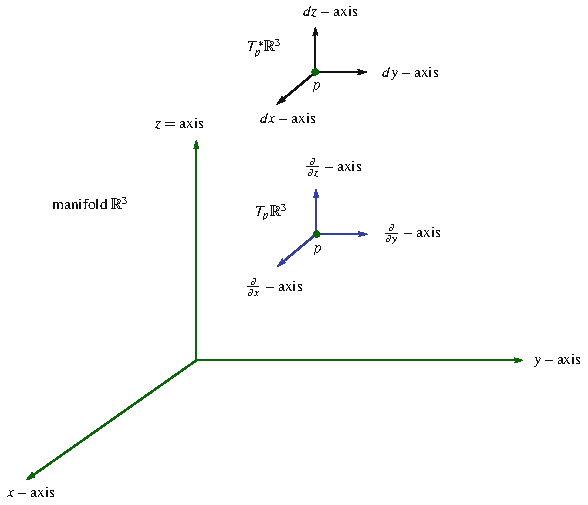
\includegraphics[width=0.715\linewidth]{images/vector/fig-3-1.pdf}
  \caption{流形 $\mathbb{R}^3$、切空间 $T_p\mathbb{R}^3$ 与余切空间 $T_p^*\mathbb{R}^3$ 一起画出. 尽管余切空间 $T_p^*\mathbb{R}^3$ 实际上与切空间 $T_p\mathbb{R}^3$ 一样附着在流形的同一点 $p$ 处，但这里把它画在切空间的上方. 本书将大体遵循这一约定}
  \label{fig:3-1}
\end{figure}

在上一章我们还发现，每个点 $p$ 处的切空间 $T_p\mathbb{R}^n$ 有一组基
\[
\left\{\left.\frac{\partial}{\partial x_1}\right|_p,\;\left.\frac{\partial}{\partial x_2}\right|_p,\ldots,\left.\frac{\partial}{\partial x_n}\right|_p\right\}
\]
并且每个点 $p$ 处有一个余切空间 $T_p^*\mathbb{R}^n$，它是向量空间 $T_p\mathbb{R}^n$ 的对偶空间，有一组基
\[
\{dx_1(p),dx_2(p),\ldots,dx_n(p)\}
\]
如果记号中省略基点 $p$，就简写为 $\{dx_1,dx_2,\ldots,dx_n\}$. 到目前为止我们建立起来的图像如图 \ref{fig:3-1} 所示，图中画出了流形 $\mathbb{R}^3$ 及其上叠加的切空间 $T_p\mathbb{R}^3$. 余切空间 $T_p^*\mathbb{R}^3$ 画在切空间的上方.

1-形式 $dx_1(p),dx_2(p),\ldots,dx_n(p)$ 恰好就是向量空间 $T_p\mathbb{R}^n$ 上的线性泛函. 与上面一致，我们有 $T_p\mathbb{R}^n\simeq\mathbb{R}^n$，其中 $T_p\mathbb{R}^n$ 的元素 $v_p$ 通常写成列向量；而 $T_p^*\mathbb{R}^n\simeq\mathbb{R}^n$，其中 $T_p^*\mathbb{R}^n$ 的元素 $\alpha_p$ 常写成行向量并称为余向量. 因此，我们可以用矩阵乘法（行向量乘以列向量）来表示 1-形式 $\alpha_p$ 作用于向量 $v_p$，即 $\alpha_p(v_p)$. 现在我们再引入一点点记号. 这有时也被写为
\[
\alpha_p(v_p)=\langle\alpha_p,v_p\rangle=\langle\alpha,v\rangle_p.
\]
因此，尖括号 $\langle\cdot,\cdot\rangle$ 表示微分形式与向量之间的\newterm{canonical-pairing}{典范配对}{canonical pairing}. 有时作者甚至不在乎典范配对中的顺序，你甚至偶尔会看到 $\langle v_p,\alpha_p\rangle$. 有些微积分教材用尖括号表示行向量；我们在这里不使用那种记号.

点 $p$ 处的微分 1-形式就是 $T_p^*\mathbb{R}^n$ 的一个元素. 我们的目标是弄清楚如何把 1-形式相乘而得到 2-形式、3-形式与 $k$-形式. 我们希望以一种能保持某些与体积有关的性质的方式来相乘微分 1-形式. （这一点一会儿就会更清楚.）

暂时我们将在流形 $\mathbb{R}^3$ 上工作，因为相关的图更容易画出. 然后我们将转向 $\mathbb{R}^2$，甚至 $\mathbb{R}$，最后再转向更一般的 $\mathbb{R}^n$ 情形. 首先我们回顾上一章所学的内容. 图 \ref{fig:3-2} 展示了线性泛函，即对偶基元素 $dx_1,dx_2,dx_3$（即 $dx,dy,dz$）对向量 $v_p\in T_p\mathbb{R}^3$ 做了什么；它们求出 $v_p$ 在 $T_p\mathbb{R}^3$ 的各坐标轴上的投影. 一般地，基点 $p$ 在记号中大部分时候被省略.

\begin{figure}[htbp]
  \centering
  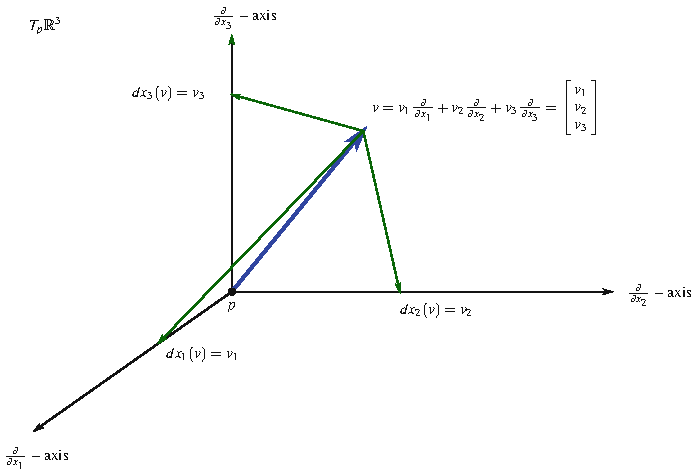
\includegraphics[width=0.845\linewidth]{images/vector/fig-3-2.pdf}
  \caption{对偶基元素如何作用于向量 $v$ 的示意图. 图中记号省略了点 $p$}
  \label{fig:3-2}
\end{figure}

图 \ref{fig:3-3} 的上方把 1-形式 $\alpha=\alpha_1dx+\alpha_2dy+\alpha_3dz$ 作为余切空间 $T_p^*\mathbb{R}^3$ 的一个元素画出. 下方展示该 1-形式作用于向量 $v_p\in T_p\mathbb{R}^3$ 的结果. 每个基元素 $dx,dy,dz$ 求出 $v$ 在相应轴上的投影. $v$ 在 $x$-轴上的投影由 $dx(v)=v_1$ 给出，然后被 $\alpha_1$ 缩放（即相乘）. $v$ 在 $y$-轴上的投影由 $dy(v)=v_2$ 给出，然后被 $\alpha_2$ 相乘. $v$ 在 $z$-轴上的投影由 $dz(v)=v_3$ 给出，然后被 $\alpha_3$ 相乘. 这三个缩放后的项 $\alpha_1v_1,\alpha_2v_2,\alpha_3v_3$ 随后相加，得到 $\alpha(v)=\alpha_1v_1+\alpha_2v_2+\alpha_3v_3$.

\begin{figure}[htbp]
  \centering
  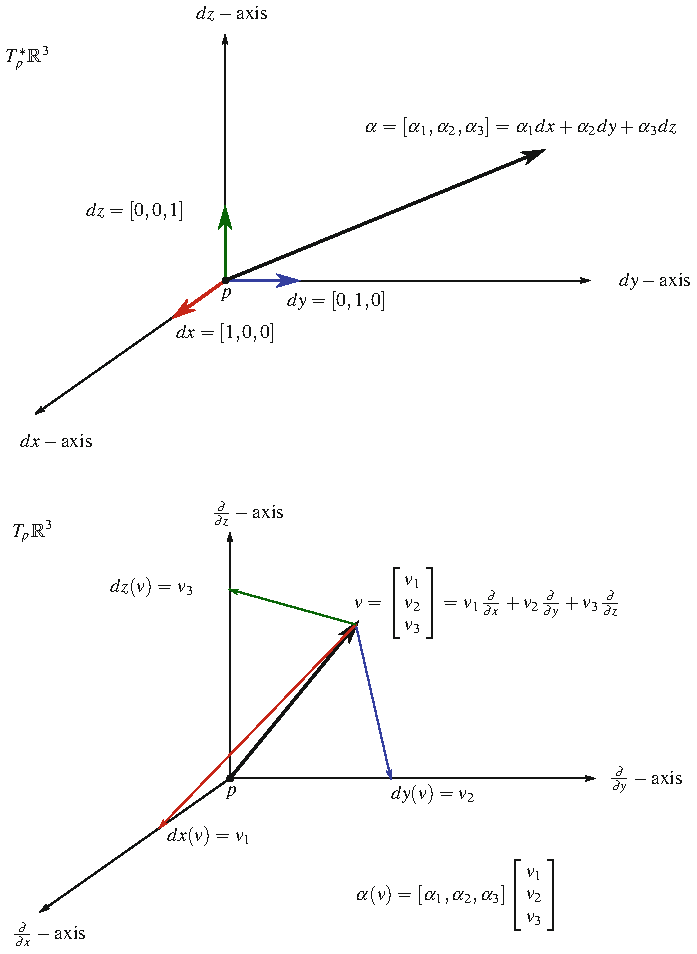
\includegraphics[width=0.826\linewidth]{images/vector/fig-3-3.pdf}
  \caption{上方，1-形式 $\alpha=\alpha_1dx+\alpha_2dy+\alpha_3dz$ 作为余切空间 $T_p^*\mathbb{R}^3$ 的元素画出. 下方，画出该 1-形式作用于向量 $v_p\in T_p\mathbb{R}^3$ 的结果}
  \label{fig:3-3}
\end{figure}

例如，由于
\[
dx_1(v_p)=dx_1\left(\begin{bmatrix}v_1\\v_2\\v_3\end{bmatrix}\right)=v_1
\]
我们可以把 $dx_1$ 看作求出向量 $v_p$ 在 $T_p\mathbb{R}^3$ 的 $\left.\frac{\partial}{\partial x_1}\right|_p$ 坐标轴上的投影. 对 $dx_2$ 与 $dx_3$ 也类似. 换言之，$dx_1$ 求出沿 $\left.\frac{\partial}{\partial x_1}\right|_p$ 坐标轴的长度. 而长度不就是一维的``体积''吗？我们希望两个 1-形式的乘积也做类似的事情，求出一个二维投影的体积. 最终这将意味着两个 1-形式的乘积将不再是 1-形式，甚至不再是线性泛函. 也就是说，它将不再是 $T_p^*\mathbb{R}^3$ 的元素，而是某种不同的东西，我们将称之为\newterm{two-form}{2-形式}{two-form}. 我们把 $\mathbb{R}^3$ 上的 2-形式空间记为 $\Lambda^2(\mathbb{R}^3)$.

在这里我们努力做到记号上非常精确，并弄清楚各个对象属于什么空间. 很容易看出混淆是如何产生的. 以图 \ref{fig:3-4} 为向导，考虑向量
\[
\begin{bmatrix}dx_1(v_p)\\dx_2(v_p)\\0\end{bmatrix}_p\in T_p\mathbb{R}^3.
\]
这个向量位于 $\mathbb{R}^3$ 在点 $p$ 处的切空间中. 换言之，它在 $T_p\mathbb{R}^3$ 中. 但这个向量也是 $v_p$ 在 $T_p\mathbb{R}^3$ 的 $\left.\frac{\partial}{\partial x_1}\right|_p\left.\frac{\partial}{\partial x_2}\right|_p$-平面上的投影. 因此我们可以把它等同于向量
\[
\binom{dx_1(v_p)}{dx_2(v_p)}_p\in\mathrm{span}\left\{\left.\frac{\partial}{\partial x_1}\right|_p,\left.\frac{\partial}{\partial x_2}\right|_p\right\}\subset T_p\mathbb{R}^3.
\]
这个向量一般被称为 $v_p$ 在 $T_p\mathbb{R}^3$ 的 $\left.\frac{\partial}{\partial x_1}\right|_p\left.\frac{\partial}{\partial x_2}\right|_p$-平面上的投影.

\begin{figure}[htbp]
  \centering
  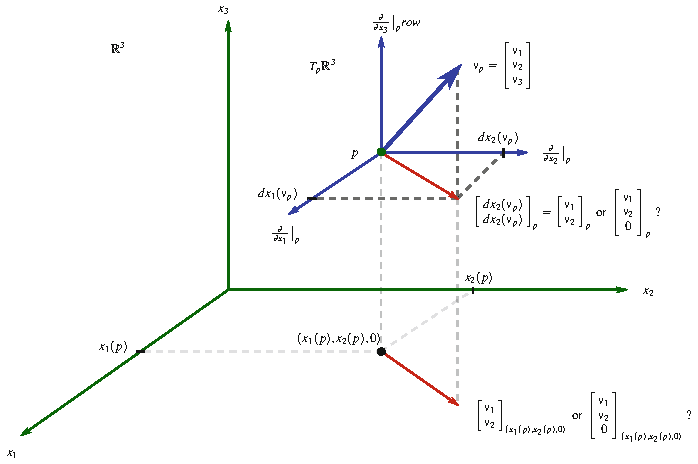
\includegraphics[width=0.960\linewidth]{images/vector/fig-3-4.pdf}
  \caption{混为一谈}
  \label{fig:3-4}
\end{figure}

再次以图 \ref{fig:3-4} 为向导来看. 注意，如果我们不够精确，就很容易把切空间中的向量
\[
\begin{bmatrix}dx_1(v_p)\\dx_2(v_p)\\0\end{bmatrix}_p\in T_p\mathbb{R}^3
\]
与 $T_p\mathbb{R}^3$ 的 $\left.\frac{\partial}{\partial x_1}\right|_p\left.\frac{\partial}{\partial x_2}\right|_p$-平面中的向量
\[
\binom{dx_1(v_p)}{dx_2(v_p)}\in T_p\mathbb{R}^3\text{ 的 }\left.\frac{\partial}{\partial x_1}\right|_p\left.\frac{\partial}{\partial x_2}\right|_p\text{-平面}
\]
与流形 $\mathbb{R}^3$ 中位于点 $p$ 处的向量
\[
\begin{bmatrix}dx_1(v_p)\\dx_2(v_p)\\0\end{bmatrix}_p\in\mathbb{R}^3
\]
甚至与流形 $\mathbb{R}^3$ 中位于点 $(x_1(p),x_2(p),0)$ 处的向量
\[
\begin{bmatrix}dx_1(v_p)\\dx_2(v_p)\\0\end{bmatrix}_{(x_1(p),x_2(p),0)}\in\mathbb{R}^3
\]
或者与 $\mathbb{R}^3$ 的 $xy$-平面中位于点 $(x_1(p),x_2(p),0)$ 处的向量
\[
\binom{dx_1(v_p)}{dx_2(v_p)}_{(x_1(p),x_2(p),0)}\in\mathbb{R}^3\text{ 的 }xy\text{-平面}
\]
混为一谈. 就 $\mathbb{R}^3$ 或 $\mathbb{R}^n$ 而言，这可能会在我们的头脑中造成混乱，但一般不会导致任何计算上的问题，这就是为什么在向量微积分中一般不做这种精确的区分. 但一般情况下我们根本不能这样做.

既然我们花了一些力气来理解各个向量所在的空间，我们就把注意力转回最初的问题：寻找两个 1-形式的乘积，使它做与 1-形式类似的事情，即求出某种体积. 正如 1-形式 $dx_1$ 输入一个向量 $v_p$ 并输出一维体积一样，我们希望两个 1-形式（比如 $dx_1$ 与 $dx_2$）的乘积输入两个向量 $v_p$ 与 $w_p$，并输出一个二维体积. 它应该给出什么体积呢？考虑图 \ref{fig:3-5}.

\begin{figure}[htbp]
  \centering
  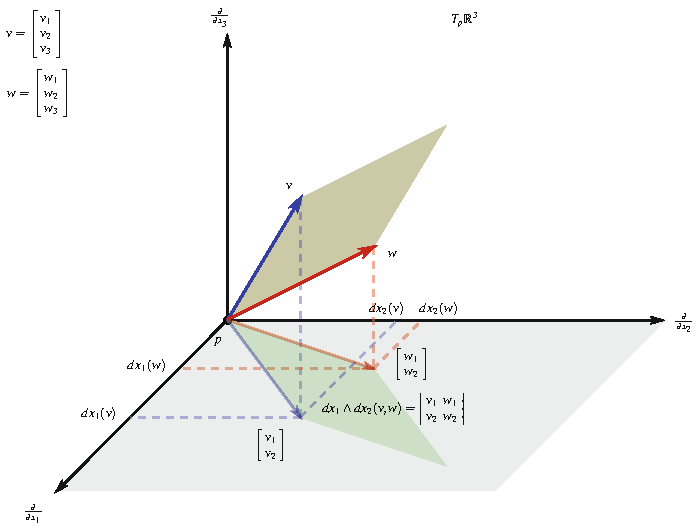
\includegraphics[width=0.960\linewidth]{images/vector/fig-3-5.pdf}
  \caption{由 $v$ 与 $w$（棕色）张成的平行六面体被投影到 $T_p\mathbb{R}^3$ 中的 $\partial x_1\partial x_2$-平面（绿色）上. 我们希望 $dx_1\wedge dx_2$ 求出这个投影区域的体积}
  \label{fig:3-5}
\end{figure}

我们已画出向量
\[
v_p=\begin{bmatrix}v_1\\v_2\\v_3\end{bmatrix}\qquad\text{与}\qquad w_p=\begin{bmatrix}w_1\\w_2\\w_3\end{bmatrix}
\]
在 $T_p\mathbb{R}^3$ 的 $\partial x_1\partial x_2$-平面上的投影. 注意我们改变了记号，把 $\left.\frac{\partial}{\partial x_i}\right|_p$ 写成了 $\partial x_i$. $v_p$ 在 $\partial x_1\partial x_2$-平面上的投影由向量
\[
\binom{dx_1(v_p)}{dx_2(v_p)}=\binom{v_1}{v_2}
\]
给出. 类似地，$w_p$ 在同一平面上的投影由
\[
\binom{dx_1(w_p)}{dx_2(w_p)}=\binom{w_1}{w_2}
\]
给出. 我们可能想要的体积中最自然的一个，是 $T_p\mathbb{R}^3$ 中 $\partial x_1\partial x_2$-平面内由这两个投影向量
\[
\binom{dx_1(v_p)}{dx_2(v_p)}\qquad\text{与}\qquad\binom{dx_1(w_p)}{dx_2(w_p)}
\]
张成的平行六面体的体积. 所以，我们希望这两个 1-形式 $dx_1$ 与 $dx_2$ 的这种``乘法''或``乘积''在输入两个向量 $v_p$ 与 $w_p$ 时能给出这个投影体积.

为了提醒我们自己这种乘法实际上不同于我们迄今为止所习惯的任何东西，我们将为它使用一种特殊的记号，称为楔号 $\wedge$，并给它起一个特别的名字，楔积. 所以，这就是我们想要的
\[
dx_1\wedge dx_2(v_p,w_p)=\text{由 }v_p\text{ 与 }w_p\text{ 在 }\partial x_1\partial x_2\text{-平面上的投影张成的平行六面体的体积}.
\]
或者，
\[
dx_1\wedge dx_2(v_p,w_p)=\text{由 }\binom{dx_1(v_p)}{dx_2(v_p)}\text{ 与 }\binom{dx_1(w_p)}{dx_2(w_p)}\text{ 张成的平行六面体的体积}.
\]
但这正是我们在第 1 章行列式那一节推导行列式定义的方式. 由向量
\[
\binom{dx_1(v_p)}{dx_2(v_p)}\qquad\text{与}\qquad\binom{dx_1(w_p)}{dx_2(w_p)}
\]
张成的平行六面体的体积，由以这些向量为列的矩阵的行列式公式给出. 因此我们可以用行列式来帮助我们定义楔积，
\[
dx_1\wedge dx_2(v_p,w_p)\equiv
\begin{vmatrix}
dx_1(v_p) & dx_1(w_p)\\
dx_2(v_p) & dx_2(w_p)
\end{vmatrix}.
\]
总之，两个 1-形式的楔积是用相应的向量投影的行列式来定义的. 所以我们看到，体积、行列式与投影（通过 1-形式）在楔积的定义中全部混合在一起并密切相关. 更一般地，两个 1-形式 $dx_i$ 与 $dx_j$ 的楔积定义为
\[
\text{两个 1-形式的楔积：}\qquad
dx_i\wedge dx_j(v_p,w_p)\equiv
\begin{vmatrix}
dx_i(v_p) & dx_i(w_p)\\
dx_j(v_p) & dx_j(w_p)
\end{vmatrix}.
\]

继续停留在流形 $\mathbb{R}^3$ 上，让我们试着对正在发生的事情获得一幅更好的图像. 回头参考图 \ref{fig:3-5}，其中两个向量 $v$ 与 $w$ 画在某个任意点 $p$ 处的切空间 $T_p\mathbb{R}^3$ 中. （此后记号中省略点 $p$.）$v$ 与 $w$ 在 $\partial x_1\partial x_2$-平面上的投影由
\[
\binom{dx_1(v_p)}{dx_2(v_p)}=\binom{v_1}{v_2}\qquad\text{与}\qquad\binom{dx_1(w_p)}{dx_2(w_p)}=\binom{w_1}{w_2}
\]
给出. 由这些投影张成的平行六面体的面积由 $dx_1\wedge dx_2(v,w)$ 给出. 作为例子，假设
\[
v=\begin{bmatrix}1\\2\\3\end{bmatrix}\qquad\text{与}\qquad w=\begin{bmatrix}4\\5\\6\end{bmatrix}.
\]
首先我们求 $dx_1\wedge dx_2(v,w)$：
\[
dx_1\wedge dx_2\left(\begin{bmatrix}1\\2\\3\end{bmatrix},\begin{bmatrix}4\\5\\6\end{bmatrix}\right)
=\begin{vmatrix}1&4\\2&5\end{vmatrix}=(1)(5)-(4)(2)=-3.
\]
注意我们得到的面积是 $-3$. 这不应该令人惊讶，因为我们知道面积实际上是有符号的. 如果我们改求 $dx_2\wedge dx_1(v,w)$：
\[
dx_2\wedge dx_1\left(\begin{bmatrix}1\\2\\3\end{bmatrix},\begin{bmatrix}4\\5\\6\end{bmatrix}\right)
=\begin{vmatrix}2&5\\1&4\end{vmatrix}=(2)(4)-(5)(1)=3
\]
我们就得到面积 3. 有一点需要提醒，当计算 $dx_1\wedge dx_2$ 时，我们的投影向量是
\[
\binom{dx_1(v_p)}{dx_2(v_p)}=\binom{1}{2}\qquad\text{与}\qquad\binom{dx_1(w_p)}{dx_2(w_p)}=\binom{4}{5}
\]
而当计算 $dx_2\wedge dx_1$ 时，我们的投影向量是
\[
\binom{dx_2(v_p)}{dx_1(v_p)}=\binom{2}{1}\qquad\text{与}\qquad\binom{dx_2(w_p)}{dx_1(w_p)}=\binom{5}{4}
\]
它们看起来可能是不同的向量. 然而它们并不是不同的向量. 我们只是把向量的分量写成不同的顺序，仅此而已. 我们不是像通常那样先写 $x_1$ 分量，而是先写了 $x_2$ 分量.

在图 \ref{fig:3-6} 中，同样的两个向量 $v$ 与 $w$ 画在某个任意点 $p$ 处的同一个切空间 $T_p\mathbb{R}^3$ 中. （同样，此后记号中省略点 $p$.）$v$ 与 $w$ 在 $\partial x_2\partial x_3$-平面上的投影由
\[
\binom{dx_2(v_p)}{dx_3(v_p)}=\binom{v_2}{v_3}\qquad\text{与}\qquad\binom{dx_2(w_p)}{dx_3(w_p)}=\binom{w_2}{w_3}
\]
给出. 由这些投影张成的平行六面体的面积由 $dx_2\wedge dx_3(v,w)$ 给出. 继续使用同一个例子，我们求 $dx_2\wedge dx_3(v,w)$：
\[
dx_2\wedge dx_3\left(\begin{bmatrix}1\\2\\3\end{bmatrix},\begin{bmatrix}4\\5\\6\end{bmatrix}\right)
=\begin{vmatrix}2&5\\3&6\end{vmatrix}=(2)(6)-(3)(5)=-3.
\]
而 $dx_3\wedge dx_2(v,w)$ 给出
\[
dx_3\wedge dx_2\left(\begin{bmatrix}1\\2\\3\end{bmatrix},\begin{bmatrix}4\\5\\6\end{bmatrix}\right)
=\begin{vmatrix}3&6\\2&5\end{vmatrix}=(3)(5)-(6)(2)=3.
\]

\begin{figure}[htbp]
  \centering
  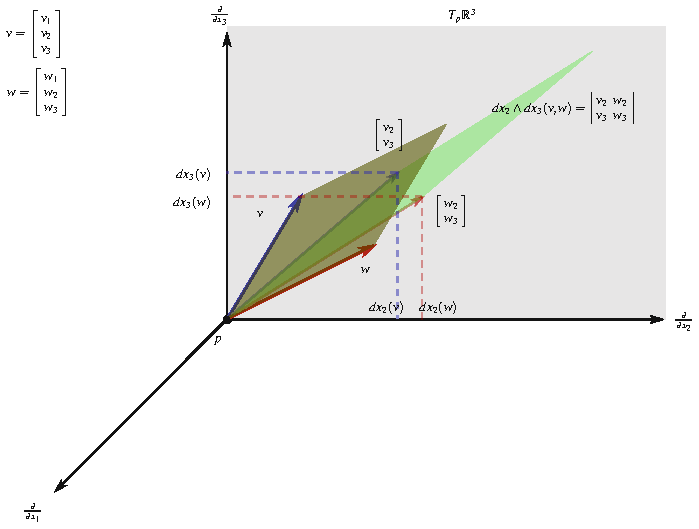
\includegraphics[width=0.960\linewidth]{images/vector/fig-3-6.pdf}
  \caption{由 $v$ 与 $w$（棕色）张成的平行六面体被投影到 $T_p\mathbb{R}^3$ 中的 $\partial x_2\partial x_3$-平面（绿色）上. 当输入向量 $v$ 与 $w$ 时，楔积 $dx_2\wedge dx_3$ 将求出该投影区域的体积}
  \label{fig:3-6}
\end{figure}

再次地，同样的两个向量 $v$ 与 $w$ 画在同一个切空间 $T_p\mathbb{R}^3$ 中，$v$ 与 $w$ 在 $\partial x_1\partial x_3$-平面上的投影由
\[
\binom{dx_1(v_p)}{dx_3(v_p)}=\binom{v_1}{v_3}\qquad\text{与}\qquad\binom{dx_1(w_p)}{dx_3(w_p)}=\binom{w_1}{w_3}
\]
给出. 这如图 \ref{fig:3-7} 所示. 由这些投影张成的平行六面体的面积由 $dx_1\wedge dx_3(v,w)$ 给出. 使用同一个例子，我们求 $dx_1\wedge dx_3(v,w)$：
\[
dx_1\wedge dx_3\left(\begin{bmatrix}1\\2\\3\end{bmatrix},\begin{bmatrix}4\\5\\6\end{bmatrix}\right)
=\begin{vmatrix}1&4\\3&6\end{vmatrix}=(1)(6)-(3)(4)=-6.
\]
而 $dx_3\wedge dx_1(v,w)$ 给出
\[
dx_3\wedge dx_1\left(\begin{bmatrix}1\\2\\3\end{bmatrix},\begin{bmatrix}4\\5\\6\end{bmatrix}\right)
=\begin{vmatrix}3&6\\1&4\end{vmatrix}=(3)(4)-(1)(6)=6.
\]

\begin{figure}[htbp]
  \centering
  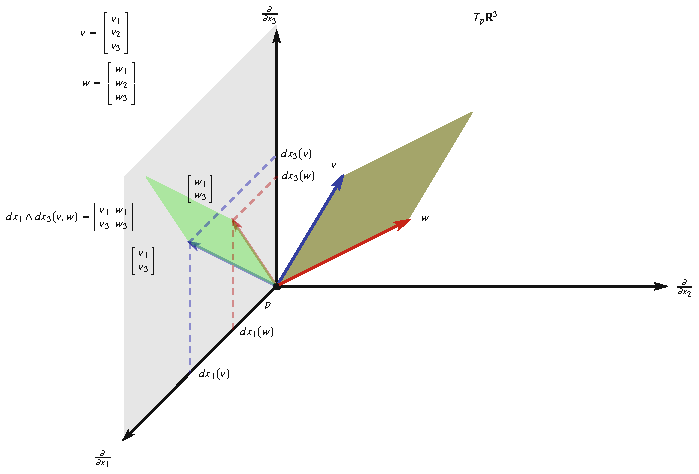
\includegraphics[width=0.960\linewidth]{images/vector/fig-3-7.pdf}
  \caption{由 $v$ 与 $w$（棕色）张成的平行六面体被投影到 $T_p\mathbb{R}^3$ 中的 $\partial x_1\partial x_3$-平面（绿色）上. 当输入向量 $v$ 与 $w$ 时，楔积 $dx_1\wedge dx_3$ 将求出该投影区域的体积}
  \label{fig:3-7}
\end{figure}

基于这些例子，看起来 $dx_i\wedge dx_j=-dx_j\wedge dx_i$. 利用上面给出的楔积定义，容易看出确实有 $dx_i\wedge dx_j=-dx_j\wedge dx_i$. 这个性质称为\newterm{skew-symmetry}{反对称性}{skew symmetry}，它由行列式的性质推出. 回忆一下，如果你交换行列式中的两行，行列式的符号就会改变. 这里发生的事情本质上就是如此. 这意味着两个 1-形式``相乘''（通过楔积）的顺序是有关系的. 如果我们交换顺序，答案就会改变一个符号.

继续使用同样的向量 $v=\begin{bmatrix}1\\2\\3\end{bmatrix}$ 与 $w=\begin{bmatrix}4\\5\\6\end{bmatrix}$，让我们求 $dx_1\wedge dx_1(v_p,w_p)$：
\[
dx_1\wedge dx_1\left(\begin{bmatrix}1\\2\\3\end{bmatrix},\begin{bmatrix}4\\5\\6\end{bmatrix}\right)
=\begin{vmatrix}1&4\\1&4\end{vmatrix}=(1)(4)-(4)(1)=0.
\]
类似地，我们有 $dx_2\wedge dx_2(v,w)=0$ 与 $dx_3\wedge dx_3(v,w)=0$. 这不应该太令人惊讶，因为一般来说我们会有
\[
dx_i\wedge dx_i(v,w)=
\begin{vmatrix}
dx_i(v) & dx_i(w)\\
dx_i(v) & dx_i(w)
\end{vmatrix}
=dx_i(v)\cdot dx_i(w)-dx_i(v)\cdot dx_i(w)=0.
\]
另一种看待这一点的方式是注意到，由 $dx_i\wedge dx_j=-dx_j\wedge dx_i$ 可以推出 $dx_i\wedge dx_i=-dx_i\wedge dx_i$，这只有当 $dx_i\wedge dx_i=0$ 时才可能发生. 遗憾的是，没有任何一幅精确的图能展示这里发生的事情. 最好就是认识到，由投影向量张成的平行六面体是退化的，因此面积为零.

所以，给定 $T_p\mathbb{R}^3$ 中的两个向量 $v_p$ 与 $w_p$，我们现在已经考虑了所有可能的两个 1-形式的楔积. 我们考虑了
\[
dx_1\wedge dx_2,\qquad dx_2\wedge dx_3,\qquad dx_1\wedge dx_3.
\]
我们还发现
\[
dx_1\wedge dx_2=-dx_2\wedge dx_1,\qquad
dx_2\wedge dx_3=-dx_3\wedge dx_2,\qquad
dx_1\wedge dx_3=-dx_3\wedge dx_1,
\]
所以一旦我们知道左边对两个向量的作用，就自动知道右边对同样这两个向量的作用. 最后，我们还发现
\[
dx_1\wedge dx_1=0,\qquad dx_2\wedge dx_2=0,\qquad dx_3\wedge dx_3=0.
\]
全部情况就是这些. 楔积 $dx_1\wedge dx_2$、$dx_2\wedge dx_3$ 与 $dx_1\wedge dx_3$ 都称为 2-形式. 事实上，每一个 2-形式都可以写成这三个 2-形式的线性组合. 例如，对任意 $a,b,c\in\mathbb{R}$，$a\,dx_1\wedge dx_2+b\,dx_2\wedge dx_3+c\,dx_1\wedge dx_3$ 都是 2-形式. 出于这个原因，2-形式 $dx_1\wedge dx_2$、$dx_2\wedge dx_3$ 与 $dx_1\wedge dx_3$ 被称为 $\mathbb{R}^3$ 上 2-形式空间的基，该空间记为 $\Lambda^2(\mathbb{R}^3)$. 实际上，有一个习惯或约定，用 2-形式 $dx_1\wedge dx_2$、$dx_2\wedge dx_3$ 与 $dx_3\wedge dx_1$ 作为 $\Lambda^2(\mathbb{R}^3)$ 的基. 我们只是把 $dx_1\wedge dx_3$ 替换成了 $dx_3\wedge dx_1$. 这样做的原因是为了在写下基时保持一种``循环次序''，而这只能在三维中做到. 但关于这一点，下一节还会详细讨论.

到目前为止我们一直在 $\mathbb{R}^3$ 上工作，因为它容易画出图像，也容易看清我们所说的投影是什么意思. 现在让我们退后一步，如图 \ref{fig:3-8} 所示，花一点时间思考 $\mathbb{R}^2$. 向量 $v_p=\binom{v_1}{v_2}$ 在 $T_p\mathbb{R}^2$ 的一维子空间 $\partial x_1$ 上的投影由向量 $[dx_1(v_p)]=[v_1]$ 给出，$v_p$ 在子空间 $\partial x_2$ 上的投影由向量 $[dx_2(v_p)]=[v_2]$ 给出，如图所示.

\begin{figure}[htbp]
  \centering
  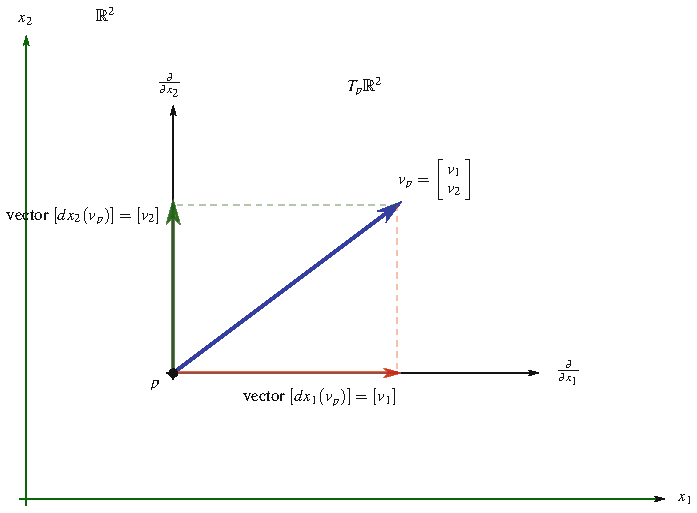
\includegraphics[width=0.826\linewidth]{images/vector/fig-3-8.pdf}
  \caption{流形 $\mathbb{R}^2$ 及其上叠加的切空间 $T_p\mathbb{R}^2$. 向量 $v_p$ 是切空间 $T_p\mathbb{R}^2$ 的一个元素}
  \label{fig:3-8}
\end{figure}

但现在考虑图 \ref{fig:3-9}. 它与图 \ref{fig:3-8} 类似，只是现在有两个向量 $v_p$ 与 $w_p$ 位于 $T_p\mathbb{R}^2$ 中，它们张成一个平行六面体. 在这里 $dx_1\wedge dx_2(v_p,w_p)$ 表示什么呢？在这种情况下 $v_p$ 与 $w_p$ 被投影到什么空间呢？我们有
\[
dx_1\wedge dx_2(v_p,w_p)
=\begin{vmatrix}
dx_1(v_p) & dx_1(w_p)\\
dx_2(v_p) & dx_2(w_p)
\end{vmatrix}
=\begin{vmatrix}
v_1 & w_1\\
v_2 & w_2
\end{vmatrix}
=v_1w_2-w_1v_2
\]
这正是由
\[
\binom{dx_1(v_p)}{dx_2(v_p)}=\binom{v_1}{v_2}=v_p
\qquad\text{与}\qquad
\binom{dx_1(w_p)}{dx_2(w_p)}=\binom{w_1}{w_2}=w_p
\]
张成的平行六面体的面积，所以 $v_p$ 与 $w_p$ 被``投影''到的空间是整个空间 $T_p\mathbb{R}^2$.

\begin{figure}[htbp]
  \centering
  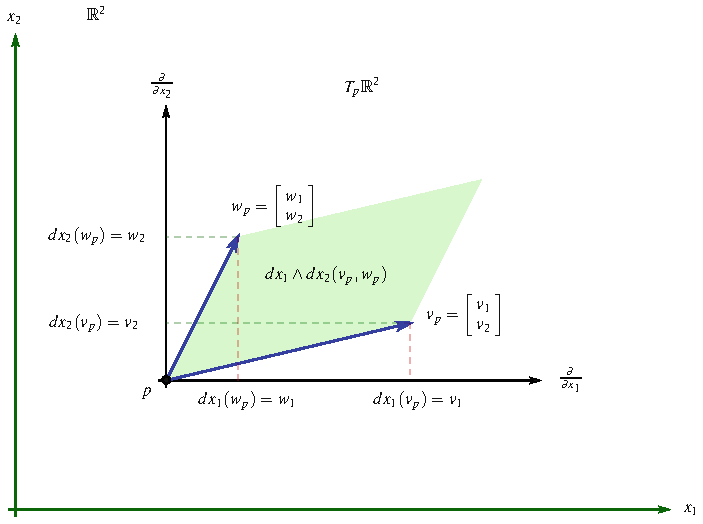
\includegraphics[width=0.833\linewidth]{images/vector/fig-3-9.pdf}
  \caption{流形 $\mathbb{R}^2$ 及其上叠加的切空间 $T_p\mathbb{R}^2$. 由 $v_p$ 与 $w_p$ 张成的平行六面体已画出. 但当 $dx_1\wedge dx_2$ 作用于向量 $v_p$ 与 $w_p$ 时，它会被投影到什么空间呢？它被投影到它已经所在的空间，即 $T_p\mathbb{R}^2$}
  \label{fig:3-9}
\end{figure}

\begin{question}\label{q:3-1}
求 $dx_2\wedge dx_1(v_p,w_p)$. 它与 $dx_1\wedge dx_2(v_p,w_p)$ 有何关系？$\Lambda_p^2(\mathbb{R}^2)$ 的基是什么？$\Lambda_p^2(\mathbb{R}^2)$ 的一般元素长什么样？
\end{question}

\begin{question}\label{q:3-2}
目前我们继续停留在 $\mathbb{R}^2$ 的例子中.
\begin{enumerate}
  \item[(a)] 考虑 $dx_1\wedge dx_2\wedge dx_1$. 你认为它需要几个向量作为输入？
  \item[(b)] 在二维空间中，由三个向量张成的平行六面体的三维体积是多少？
  \item[(c)] 设 $u=\binom{u_1}{u_2}$、$v=\binom{v_1}{v_2}$、$s=\binom{w_1}{w_2}$，并设
  \[
  dx_1\wedge dx_2\wedge dx_1(u,v,w)\equiv
  \begin{vmatrix}
  dx_1(u) & dx_1(v) & dx_1(w)\\
  dx_2(u) & dx_2(v) & dx_2(w)\\
  dx_1(u) & dx_1(v) & dx_1(w)
  \end{vmatrix}.
  \]
  解释为什么它总是零.
  \item[(d)] 基于此，你认为空间 $\Lambda_p^3(\mathbb{R}^2)$ 会是什么？
  \item[(e)] 基于此，你认为当 $n>3$ 时空间 $\Lambda_p^n(\mathbb{R}^2)$ 会是什么？
\end{enumerate}
\end{question}

我们把三个 1-形式的楔积定义如下：
\[
\text{三个 1-形式的楔积：}\qquad
dx_i\wedge dx_j\wedge dx_k(u,v,w)\equiv
\begin{vmatrix}
dx_i(u) & dx_i(v) & dx_i(w)\\
dx_j(u) & dx_j(v) & dx_j(w)\\
dx_k(u) & dx_k(v) & dx_k(w)
\end{vmatrix}.
\]
我们将三个 1-形式 $dx_i\wedge dx_j\wedge dx_k$ 的楔积称为\newterm{three-form}{3-形式}{three-form}. 这个 3-形式 $dx_i\wedge dx_j\wedge dx_k$ 求出什么呢？假设我们在流形 $\mathbb{R}^n$ 上. 给定点 $p$ 处的向量 $u,v,w$，我们首先求出这些向量在 $T_p\mathbb{R}^n$ 的 $\partial x_i\partial x_j\partial x_k$-子空间上的投影. 这些投影由向量
\[
\begin{bmatrix}dx_i(u)\\dx_j(u)\\dx_k(u)\end{bmatrix},\qquad
\begin{bmatrix}dx_i(v)\\dx_j(v)\\dx_k(v)\end{bmatrix},\qquad
\begin{bmatrix}dx_i(w)\\dx_j(w)\\dx_k(w)\end{bmatrix}
\]
给出.

接下来，我们利用行列式求出由这些投影向量张成的平行六面体的体积. 回到 $\mathbb{R}^3$，我们考虑 3-形式 $dx_1\wedge dx_2\wedge dx_3$. 3-形式 $dx_1\wedge dx_2\wedge dx_3$ 投影到 $T_p\mathbb{R}^3$ 的什么子空间上呢？3-形式 $dx_1\wedge dx_2\wedge dx_3$ 投影到整个空间 $T_p\mathbb{R}^3$ 上. 因此 3-形式 $dx_1\wedge dx_2\wedge dx_3$ 只是求出由三个输入向量张成的平行六面体的体积，见图 \ref{fig:3-10}.

\begin{figure}[htbp]
  \centering
  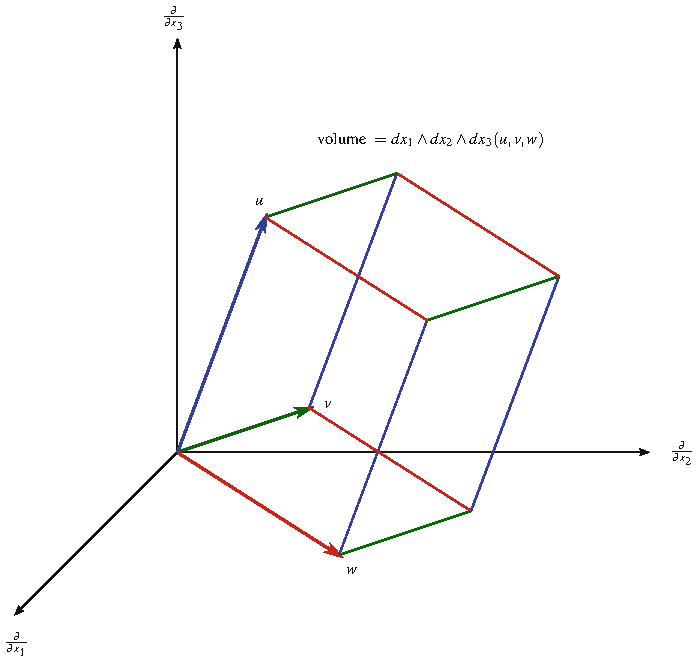
\includegraphics[width=0.829\linewidth]{images/vector/fig-3-10.pdf}
  \caption{切空间 $T_p\mathbb{R}^3$ 及由 $u$、$v$、$w$ 张成的平行六面体. 3-形式 $dx_1\wedge dx_2\wedge dx_3$（这里写为 $dx\wedge dy\wedge dz$）只是求出该平行六面体的体积}
  \label{fig:3-10}
\end{figure}

\begin{question}\label{q:3-3}
考虑流形 $\mathbb{R}^3$ 与 3-形式 $dx_1\wedge dx_2\wedge dx_3$.
\begin{enumerate}
  \item[(a)] $dx_1\wedge dx_2\wedge dx_3$ 与 $dx_2\wedge dx_1\wedge dx_3$ 有何关系？与 $dx_2\wedge dx_3\wedge dx_1$ 呢？或者 $dx_3\wedge dx_2\wedge dx_1$ 呢？你注意到什么规律了吗？
  \item[(b)] $\Lambda_p^3(\mathbb{R}^3)$ 的基是什么？
  \item[(c)] 你认为 $dx_1\wedge dx_2\wedge dx_3\wedge dx_1(u,v,w,x)$ 会如何定义？你认为它会是什么？为什么？（这里的输入 $x$ 表示第四个向量.）
  \item[(d)] 当 $n\geq4$ 时，$\Lambda_p^n(\mathbb{R}^3)$ 是什么？
\end{enumerate}
\end{question}

一般地，设 $v_1,v_2,\ldots,v_n$ 表示向量，我们把 $n$ 个 1-形式的楔积定义如下：
\[
\text{楔积（n 个 1-形式）：}\\[2mm]
dx_{i_1}\wedge dx_{i_2}\wedge\cdots\wedge dx_{i_n}(v_1,v_2,\ldots,v_n)\equiv
{\setlength{\arraycolsep}{0.5pt}\begin{vmatrix}
dx_{i_1}(v_1) & dx_{i_1}(v_2) & \cdots & dx_{i_1}(v_n)\\
dx_{i_2}(v_1) & dx_{i_2}(v_2) & \cdots & dx_{i_2}(v_n)\\
\vdots & \vdots & \ddots & \vdots\\
dx_{i_n}(v_1) & dx_{i_n}(v_2) & \cdots & dx_{i_n}(v_n)
\end{vmatrix}}.
\]
注意，如果任意两个 1-形式相同，即对某个 $j\neq k$ 有 $i_j=i_k$，那么我们就有两行相同，这给出值零.

为了结束本节，我们将考虑流形 $\mathbb{R}$ 上的 1-形式 $dx$、流形 $\mathbb{R}^2$ 上的 2-形式 $dx_1\wedge dx_2$、流形 $\mathbb{R}^3$ 上的 3-形式 $dx_1\wedge dx_2\wedge dx_3$，以及流形 $\mathbb{R}^n$ 上的 n-形式 $dx_1\wedge dx_2\wedge\cdots\wedge dx_n$. 这些是非常特殊的微分形式，通常被称为\newterm{volume-form}{体积形式}{volume form}，不过在二维情形中，2-形式 $dx_1\wedge dx_2$ 也常被称为\newterm{area-form}{面积形式}{area form}. 学完本节之后，这个术语背后的原因是相当明显的. 1-形式 $dx$ 求出 $\mathbb{R}$ 上向量的一维体积，即长度. 类似地，2-形式 $dx_1\wedge dx_2$（也写为 $dx\wedge dy$）求出 $\mathbb{R}^2$ 上平行六面体的二维体积，即面积（图 \ref{fig:3-9}）；3-形式 $dx_1\wedge dx_2\wedge dx_3$（也写为 $dx\wedge dy\wedge dz$）求出 $\mathbb{R}^3$ 上平行六面体的三维体积（图 \ref{fig:3-10}）；显然 n-形式 $dx_1\wedge dx_2\wedge\cdots\wedge dx_n$ 求出 $\mathbb{R}^n$ 上平行六面体的 n 维体积. 严格地说，被求体积的平行六面体实际上位于某个切空间中而不是流形中，但对于欧几里得空间，我们实际上也可以想象平行六面体位于流形本身中，所以我们就不在这个问题上过分纠缠了. 当我们讲到形式的积分时，这些体积形式将扮演至关重要的角色.

\begin{question}\label{q:3-4}
考虑 n-形式 $dx_{i_1}\wedge dx_{i_2}\wedge\cdots\wedge dx_{i_n}$. 如果某个 1-形式 $dx_{i_j}=dx_{i_k}$（其中 $i_j\neq i_k$）会怎样？如果某个向量 $v_j=v_k$（其中 $j\neq k$）会怎样？
\end{question}

\begin{question}\label{q:3-5}
证明：若 $i_j\neq i_k$，则交换 $dx_{i_j}$ 与 $dx_{i_k}$ 会使楔积改变符号.
\end{question}

\section{一般的 2-形式与 3-形式}

2-形式是由两个 1-形式楔乘在一起构成的. 正如我们用 $T_p^*\mathbb{R}^3$ 表示点 $p$ 处的余切空间（它是点 $p$ 处的 1-形式空间）一样，我们把点 $p$ 处的 2-形式空间记为 $\Lambda_p^2(\mathbb{R}^3)$. 与此约定一致，你偶尔会看到 $T_p^*\mathbb{R}^3$ 被写为 $\Lambda_p^1(\mathbb{R}^3)$. 正如我们已经提到的，空间 $\Lambda_p^2(\mathbb{R}^3)$ 的基由
\[
\{dx_1\wedge dx_2,\;dx_2\wedge dx_3,\;dx_3\wedge dx_1\}
\]
给出. 为什么列表中的最后一个元素写成 $dx_3\wedge dx_1$ 而不是 $dx_1\wedge dx_3$？这纯粹是基于希望循环地书写指标（index）的约定问题. 这些基元素 $dx_1\wedge dx_2$、$dx_2\wedge dx_3$、$dx_3\wedge dx_1$ 中的每一个都求出两个向量在 $T_p\mathbb{R}^3$ 的适当平面上的投影所张成的平行六面体的有向面积，如图 \ref{fig:3-11} 所示.

\begin{figure}[htbp]
  \centering
  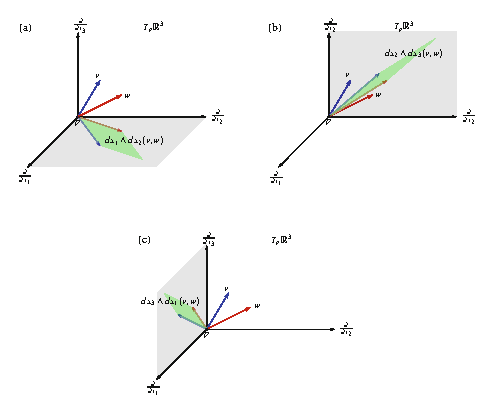
\includegraphics[width=0.880\linewidth]{images/vector/fig-3-11.pdf}
  \caption{$\Lambda^2(\mathbb{R}^3)$ 的基元素的几何作用：把 $v$ 与 $w$ 投影到 $T_p\mathbb{R}^3$ 中适当的平面上，然后求出由投影张成的平行六面体的有向面积，该面积以绿色显示. (a) $dx_1\wedge dx_2$ 的作用. (b) $dx_2\wedge dx_3$ 的作用. (c) $dx_3\wedge dx_1$ 的作用}
  \label{fig:3-11}
\end{figure}

类似地，不难看出空间 $\Lambda_p^2(\mathbb{R}^2)$ 的基由
\[
\{dx_1\wedge dx_2\}
\]
给出，而空间 $\Lambda_p^2(\mathbb{R}^4)$ 的基由
\[
\{dx_1\wedge dx_2,\;dx_1\wedge dx_3,\;dx_1\wedge dx_4,\;dx_2\wedge dx_3,\;dx_2\wedge dx_4,\;dx_3\wedge dx_4\}
\]
给出，等等. $\Lambda_p^2(\mathbb{R}^n)$ 的基含有 $\frac{n(n-1)}{2}$ 个元素.

\begin{question}\label{q:3-6}
解释为什么 $\{dx_1\wedge dx_2\}$ 是 $\Lambda_p^2(\mathbb{R}^2)$ 的基，为什么 $\{dx_1\wedge dx_2,dx_1\wedge dx_3,dx_1\wedge dx_4,dx_2\wedge dx_3,dx_2\wedge dx_4,dx_3\wedge dx_4\}$ 是 $\Lambda_p^2(\mathbb{R}^4)$ 的基.
\end{question}

\begin{question}\label{q:3-7}
解释为什么 $\Lambda_p^2(\mathbb{R}^n)$ 的基含有 $\frac{n(n-1)}{2}$ 个元素.
\end{question}

到目前为止，我们只看过 2-形式的基元素. 但空间 $\Lambda_p^2(\mathbb{R}^2)$、$\Lambda_p^2(\mathbb{R}^3)$、$\Lambda_p^2(\mathbb{R}^4)$ 或 $\Lambda_p^2(\mathbb{R}^n)$ 中的其他元素又如何呢？它们长什么样、做什么？目前我们集中讨论空间 $\Lambda_p^2(\mathbb{R}^3)$，因此将采用记号 $x,y,z$ 而不是 $x_1,x_2,x_3$.

考虑 2-形式 $5dx\wedge dy$ 作用于某个 $p$ 的两个向量 $v_p$ 与 $w_p$. 因子 5 做什么？$dx\wedge dy(v_p,w_p)$ 给出由 $v_p$ 与 $w_p$ 在 $\partial x\partial y$-平面上的投影张成的平行六面体的面积. 数字五把面积乘以五，从而缩放这个面积. 因此基元素 $dx\wedge dy$、$dy\wedge dz$、$dz\wedge dx$ 前面的数值因子是缩放因子.

图 \ref{fig:3-12} 试图展示形如 $dx\wedge dy+dy\wedge dz$ 的 2-形式对 $T_p\mathbb{R}^3$ 中两个向量 $v$ 与 $w$ 的作用. 先求出 $v$ 与 $w$ 在 $\partial x\partial y$-平面上的投影
\[
\binom{dx(v)}{dy(v)}\qquad\text{与}\qquad\binom{dx(w)}{dy(w)}
\]
并画出由这两个投影向量在 $\partial x\partial y$-平面中形成的平行六面体. $dx\wedge dy(v,w)$ 求出这个平行六面体的有向面积. 然后求出 $v$ 与 $w$ 在 $\partial y\partial z$-平面上的投影
\[
\binom{dy(v)}{dz(v)}\qquad\text{与}\qquad\binom{dy(w)}{dz(w)}
\]
并同样画出由这两个投影向量在 $\partial y\partial z$-平面中形成的平行六面体. $dy\wedge dz(v,w)$ 求出这个平行六面体的有向面积. 2-形式 $dx\wedge dy+dy\wedge dz$ 把这两个有向面积相加：
\[
\bigl(dx\wedge dy+dy\wedge dz\bigr)(v,w)=dx\wedge dy(v,w)+dy\wedge dz(v,w).
\]
形如 $adx\wedge dy+bdy\wedge dz$（其中 $a,b\in\mathbb{R}$）的 2-形式在相加之前先把平行六面体面积乘以因子 $a$ 与 $b$：
\[
\bigl(adx\wedge dy+bdy\wedge dz\bigr)(v,w)=adx\wedge dy(v,w)+bdy\wedge dz(v,w).
\]

\begin{figure}[htbp]
  \centering
  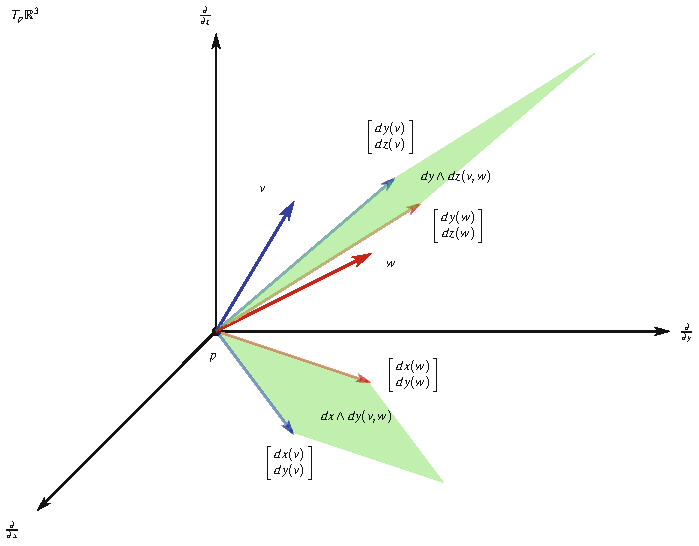
\includegraphics[width=0.944\linewidth]{images/vector/fig-3-12.pdf}
  \caption{2-形式 $dx\wedge dy+dy\wedge dz$ 对两个向量 $v$ 与 $w$ 的作用. 2-形式 $dx\wedge dy+dy\wedge dz$ 求出两个投影平行六面体的面积之和}
  \label{fig:3-12}
\end{figure}

图 \ref{fig:3-13} 表明，2-形式 $dy\wedge dz+dz\wedge dx$ 对 $T_p\mathbb{R}^3$ 中两个向量 $v$ 与 $w$ 的作用本质上是类似的. 先求出 $v$ 与 $w$ 在 $\partial y\partial z$-平面上的投影
\[
\binom{dy(v)}{dz(v)}\qquad\text{与}\qquad\binom{dy(w)}{dz(w)}
\]
并画出由这两个投影向量在 $\partial y\partial z$-平面中形成的平行六面体. $dy\wedge dz(v,w)$ 求出这个平行六面体的有向面积. 然后求出 $v$ 与 $w$ 在 $\partial x\partial z$-平面上的投影
\[
\binom{dx(v)}{dz(v)}\qquad\text{与}\qquad\binom{dx(w)}{dz(w)}
\]
并同样画出由这两个投影向量在 $\partial x\partial z$-平面中形成的平行六面体. $dz\wedge dx(v,w)$ 求出这个平行六面体的有向面积. 2-形式 $dy\wedge dz+dz\wedge dx$ 把这两个有向面积相加：
\[
\bigl(dy\wedge dz+dz\wedge dx\bigr)(v,w)=dy\wedge dz(v,w)+dz\wedge dx(v,w).
\]
形如 $ady\wedge dz+bdz\wedge dx$（其中 $a,b\in\mathbb{R}$）的 2-形式在相加之前先把平行六面体面积乘以因子 $a$ 与 $b$：
\[
\bigl(ady\wedge dz+bdz\wedge dx\bigr)(v,w)=ady\wedge dz(v,w)+bdz\wedge dx(v,w).
\]

\begin{figure}[htbp]
  \centering
  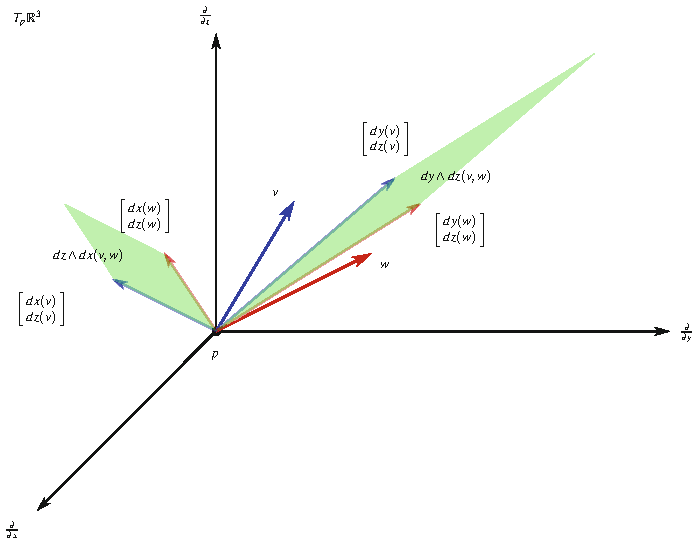
\includegraphics[width=0.944\linewidth]{images/vector/fig-3-13.pdf}
  \caption{2-形式 $dy\wedge dz+dz\wedge dx$ 对两个向量 $v$ 与 $w$ 的作用. 2-形式 $dy\wedge dz+dz\wedge dx$ 求出两个投影平行六面体的面积之和}
  \label{fig:3-13}
\end{figure}

不再重复所有细节，2-形式 $dx\wedge dy+dz\wedge dx$ 与 $adx\wedge dy+bdz\wedge dx$ 作用于两个向量 $v,w\in T_p\mathbb{R}^3$ 时的行为是类似的，见图 \ref{fig:3-14}.

\begin{figure}[htbp]
  \centering
  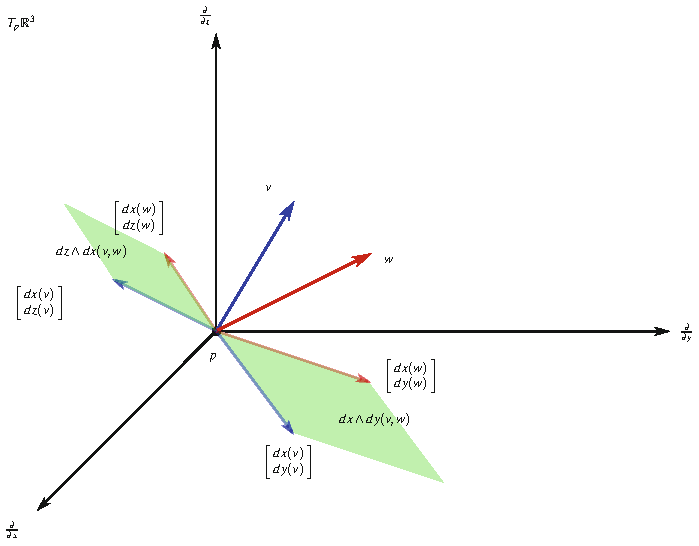
\includegraphics[width=0.944\linewidth]{images/vector/fig-3-14.pdf}
  \caption{2-形式 $dx\wedge dy+dz\wedge dx$ 对两个向量 $v$ 与 $w$ 的作用. 2-形式 $dx\wedge dy+dz\wedge dx$ 求出两个投影平行六面体的面积之和}
  \label{fig:3-14}
\end{figure}

最后，我们考虑形如 $dx\wedge dy+dy\wedge dz+dz\wedge dx$ 的 2-形式. 这种 2-形式作用于两个向量 $v,w\in T_p\mathbb{R}^3$ 的方式与你预期完全一致，如图 \ref{fig:3-15} 所示. 首先求出在 $T_p\mathbb{R}^3$ 各不同平面上的投影. 然后画出由这些投影向量形成的平行六面体. $dx\wedge dy(v,w)$ 求出 $\partial x\partial y$-平面中平行六面体的有向体积，$dy\wedge dz(v,w)$ 求出 $\partial y\partial z$-平面中平行六面体的有向体积，$dz\wedge dx(v,w)$ 求出 $\partial x\partial z$-平面中平行六面体的有向体积. 然后把这些有向体积相加：
\[
\bigl(dx\wedge dy+dy\wedge dz+dz\wedge dx\bigr)(v,w)=dx\wedge dy(v,w)+dy\wedge dz(v,w)+dz\wedge dx(v,w).
\]
形如 $adx\wedge dy+bdy\wedge dz+cdz\wedge dx$（其中 $a,b,c\in\mathbb{R}$）的 2-形式的工作方式类似，只是各个有向体积在相加之前分别被因子 $a,b,c$ 缩放.

\begin{figure}[htbp]
  \centering
  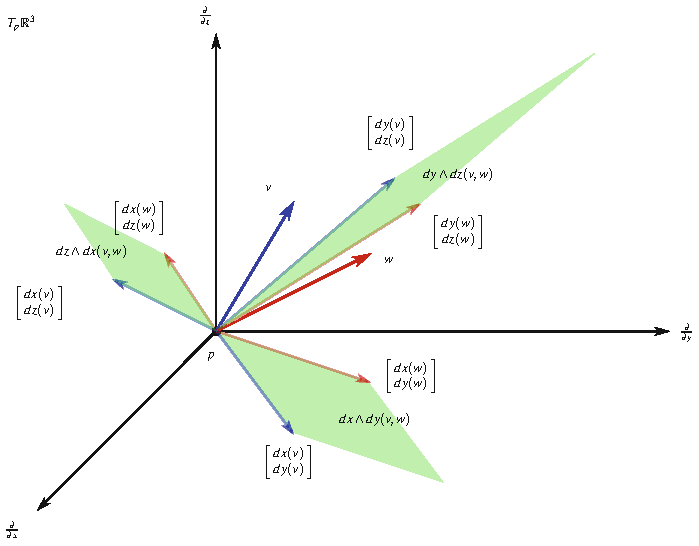
\includegraphics[width=0.944\linewidth]{images/vector/fig-3-15.pdf}
  \caption{2-形式 $dx\wedge dy+dy\wedge dz+dz\wedge dx$ 对两个未画出的向量 $v$ 与 $w$ 的作用}
  \label{fig:3-15}
\end{figure}

n 维流形（例如 $n>3$ 的 $\mathbb{R}^n$）上的 2-形式的行为完全类似. 求出两个向量 $v,w$ 在 $T_p\mathbb{R}^n$ 的适当二维子空间上的投影，由这些投影向量形成二维平行六面体，先求出它们的体积，再乘以适当的因子缩放，然后把缩放后的体积相加. 唯一的区别在于，$T_p\mathbb{R}^n$ 有 $\frac{n(n-1)}{2}$ 个不同的二维子空间.

我们已经讨论过 $\mathbb{R}^3$ 上 3-形式的空间 $\Lambda_p^3(\mathbb{R}^3)$，但为了完整起见，这里再介绍一遍. $\Lambda_p^3(\mathbb{R}^3)$ 的基由 $\{dx\wedge dy\wedge dz\}$ 给出，因为 3-形式 $dx\wedge dy\wedge dz$ 把三个向量 $u,v,w$ 投影到 $T_p\mathbb{R}^3$ 的 $\partial x\partial y\partial z$-子空间上，而这个子空间恰好是整个空间 $T_p\mathbb{R}^3$. 见图 \ref{fig:3-10}. 因此，3-形式 $dx\wedge dy\wedge dz$ 只是求出由向量 $u,v,w$ 张成的平行六面体的体积. $\Lambda_p^3(\mathbb{R}^3)$ 中形如 $adx\wedge dy\wedge dz$（其中 $a\in\mathbb{R}$）的元素只是把体积按因子 $a$ 缩放.

3-形式只在流形维数为四或更高时才开始变得有趣. 作为说明性例子，让我们考虑 $\Lambda_p^3(\mathbb{R}^4)$，即流形 $\mathbb{R}^4$ 上的 3-形式. 稍微想一想你就应该相信，$\Lambda_p^3(\mathbb{R}^4)$ 的基由
\[
\{dx_1\wedge dx_2\wedge dx_3,\;dx_1\wedge dx_2\wedge dx_4,\;dx_1\wedge dx_3\wedge dx_4,\;dx_2\wedge dx_3\wedge dx_4\}
\]
给出，并且 $\Lambda_p^3(\mathbb{R}^4)$ 的所有元素都具有
\[
adx_1\wedge dx_2\wedge dx_3+bdx_1\wedge dx_2\wedge dx_4+cdx_1\wedge dx_3\wedge dx_4+ddx_2\wedge dx_3\wedge dx_4
\]
的形式，其中 $a,b,c,d\in\mathbb{R}$.

\begin{question}\label{q:3-8}
解释为什么 $\{dx_1\wedge dx_2\wedge dx_3,dx_1\wedge dx_2\wedge dx_4,dx_1\wedge dx_3\wedge dx_4,dx_2\wedge dx_3\wedge dx_4\}$ 是 $\Lambda_p^3(\mathbb{R}^4)$ 的基. $\mathbb{R}^4$ 的所有可能的三维子空间是什么？
\end{question}

我们用来``可视化''这些 3-形式对三个向量 $u,v,w\in T_p\mathbb{R}^4$ 的作用的图像，迫于需要将是一幅``漫画''，但它足够好用；见图 \ref{fig:3-16}. 事实上，类似的漫画可以用在 m 维流形上的所有 n-形式上. 把四维向量
\[
u=\begin{bmatrix}u_1\\u_2\\u_3\\u_4\end{bmatrix},\qquad
v=\begin{bmatrix}v_1\\v_2\\v_3\\v_4\end{bmatrix},\qquad
w=\begin{bmatrix}w_1\\w_2\\w_3\\w_4\end{bmatrix}
\]
投影到 $\partial x_1\partial x_2\partial x_3$-子空间上，得到
\[
\begin{bmatrix}dx_1(u)\\dx_2(u)\\dx_3(u)\end{bmatrix}
=\begin{bmatrix}u_1\\u_2\\u_3\end{bmatrix},\qquad
\begin{bmatrix}dx_1(v)\\dx_2(v)\\dx_3(v)\end{bmatrix}
=\begin{bmatrix}v_1\\v_2\\v_3\end{bmatrix},\qquad
\begin{bmatrix}dx_1(w)\\dx_2(w)\\dx_3(w)\end{bmatrix}
=\begin{bmatrix}w_1\\w_2\\w_3\end{bmatrix}.
\]
3-形式 $dx_1\wedge dx_2\wedge dx_3(u,v,w)$ 求出由投影向量张成的平行六面体的有向体积. 3-形式 $adx_1\wedge dx_2\wedge dx_3(u,v,w)$ 按因子 $a$ 缩放该有向体积. 其他 3-形式的工作方式类似，可以用同一类漫画来想象. 最后，$\Lambda_p^3(\mathbb{R}^4)$ 的任意元素求出适当的有向体积，按适当的因子缩放这些有向体积，然后按照
\[
\bigl(adx_1\wedge dx_2\wedge dx_3+bdx_1\wedge dx_2\wedge dx_4+cdx_1\wedge dx_3\wedge dx_4+ddx_2\wedge dx_3\wedge dx_4\bigr)(u,v,w)
\]
\begin{align*}
&=adx_1\wedge dx_2\wedge dx_3(u,v,w)+bdx_1\wedge dx_2\wedge dx_4(u,v,w)\\
&\quad+cdx_1\wedge dx_3\wedge dx_4(u,v,w)+ddx_2\wedge dx_3\wedge dx_4(u,v,w)
\end{align*}
把结果相加.

\begin{figure}[htbp]
  \centering
  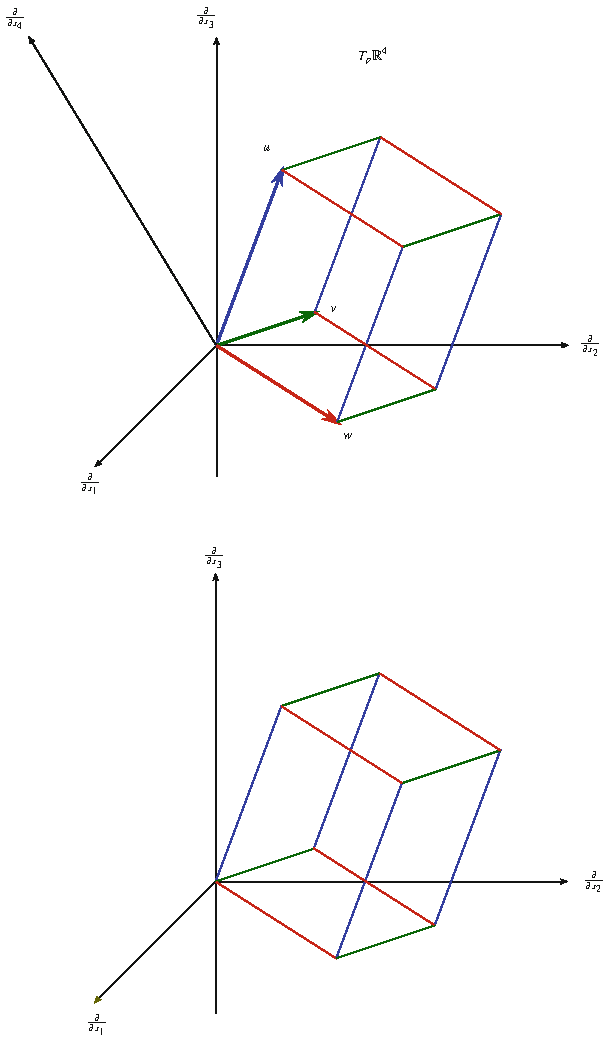
\includegraphics[width=0.729\linewidth]{images/vector/fig-3-16.pdf}
  \caption{图中试图说明切空间 $T_p\mathbb{R}^4$，并画出由 $v_1,v_2,v_3$ 张成的平行六面体（上方）. 3-形式 $dx_1\wedge dx_2\wedge dx_3$ 对三个向量 $u,v,w$ 的作用被表示为该平行六面体到三维 $\partial x_1\partial x_2\partial x_3$ 子空间的投影（下方）}
  \label{fig:3-16}
\end{figure}

\begin{question}\label{q:3-9}
考虑流形 $\mathbb{R}^3$.
\begin{enumerate}
  \item[(a)] 下列哪些是 $\mathbb{R}^3$ 上的 1-形式？
  \begin{enumerate}
    \item[(i)] $3dx_1$
    \item[(ii)] $-4dx_2+7dx_3$
    \item[(iii)] $5dx_1+3dx_2-6dx_1+4dx_3$
    \item[(iv)] $2dx_1\wedge dx_2-4dx_3$
    \item[(v)] $dx_1\wedge dx_2-3dx_2\wedge dx_3$
  \end{enumerate}
  \item[(b)] 下列哪些是 $\mathbb{R}^3$ 上的 2-形式？
  \begin{enumerate}
    \item[(i)] $-4dx_3\wedge dx_2\wedge dx_1$
    \item[(ii)] $6dx_3\wedge dx_2+8dx_3$
    \item[(iii)] $-10dx_1\wedge dx_3+5dx_2\wedge dx_3-dx_1\wedge dx_2$
    \item[(iv)] $-2dx_1\wedge dx_2+3dx_3\wedge dx_2\wedge dx_1$
    \item[(v)] $3dx_1\wedge dx_3-dx_2\wedge dx_3$
  \end{enumerate}
  \item[(c)] 下列哪些是 $\mathbb{R}^3$ 上的 3-形式？
  \begin{enumerate}
    \item[(i)] $5dx_3\wedge dx_2\wedge dx_1$
    \item[(ii)] $-3dx_3\wedge dx_2+2dx_3\wedge dx_1\wedge dx_2$
    \item[(iii)] $5dx_2\wedge dx_3\wedge dx_1+5dx_1\wedge dx_3\wedge dx_2-dx_1\wedge dx_2\wedge dx_3$
    \item[(iv)] $-5dx_3\wedge dx_2+3dx_1\wedge dx_2-dx_3\wedge dx_1$
    \item[(v)] $9dx_1-7dx_2\wedge dx_3$
  \end{enumerate}
\end{enumerate}
\end{question}

\section{n-形式的楔积}

既然我们知道了楔积在几何上做什么，我们就希望能够用代数公式快速处理形式的楔积. 本节我们学习与微分形式有关的一些代数. 首先我们将看到，微分形式基本上遵循我们期望的代数规则，只需稍作调整以适应 $dx_i\wedge dx_j=-dx_j\wedge dx_i$ 这一事实. 之后我们将介绍一点常用记号，然后写出楔积的一个一般公式.

\subsection{代数性质}

设 $\omega,\omega_1,\omega_2$ 是 k-形式，$\eta,\eta_1,\eta_2$ 是 $\ell$-形式. 那么下列性质成立：

\begin{property}{1}\label{prop:3-1}
$(a\omega)\wedge\eta=\omega\wedge(a\eta)=a(\omega\wedge\eta)$，其中 $a\in\mathbb{R}$.
\end{property}

\begin{property}{2}\label{prop:3-2}
$(\omega_1+\omega_2)\wedge\eta=\omega_1\wedge\eta+\omega_2\wedge\eta$.
\end{property}

\begin{property}{3}\label{prop:3-3}
$\omega\wedge(\eta_1+\eta_2)=\omega\wedge\eta_1+\omega\wedge\eta_2$.
\end{property}

\begin{property}{4}\label{prop:3-4}
$\omega\wedge\eta=(-1)^{k\ell}\eta\wedge\omega$.
\end{property}

我们首先通过看 $\mathbb{R}^3$ 上几个简单的例子来说明这些代数性质是合理的. 我们从第一条性质开始，证明 $(adx_1)\wedge dx_2=dx_1\wedge(adx_2)=a(dx_1\wedge dx_2)$. 首先我们有
\begin{align*}
(adx_1)\wedge dx_2(u,v)
&=\begin{vmatrix}
adx_1(u) & adx_1(v)\\
dx_2(u) & dx_2(v)
\end{vmatrix}\\
&=adx_1(u)dx_2(v)-adx_1(v)dx_2(u)\\
&=a\bigl(dx_1(u)dx_2(v)-dx_1(v)dx_2(u)\bigr)\\
&=a\begin{vmatrix}
dx_1(u) & dx_1(v)\\
dx_2(u) & dx_2(v)
\end{vmatrix}\\
&=a\bigl(dx_1\wedge dx_2\bigr)(u,v).
\end{align*}
类似地，
\begin{align*}
dx_1\wedge(adx_2)(u,v)
&=\begin{vmatrix}
dx_1(u) & dx_1(v)\\
adx_2(u) & adx_2(v)
\end{vmatrix}\\
&=adx_1(u)dx_2(v)-adx_1(v)dx_2(u)\\
&=a\bigl(dx_1(u)dx_2(v)-dx_1(v)dx_2(u)\bigr)\\
&=a\begin{vmatrix}
dx_1(u) & dx_1(v)\\
dx_2(u) & dx_2(v)
\end{vmatrix}\\
&=a\bigl(dx_1\wedge dx_2\bigr)(u,v).
\end{align*}
把所有这一切放在一起，不写出向量，就得到我们想要的恒等式. 接下来看一个说明第二条性质的例子；我们证明 $(dx_1+dx_2)\wedge dx_3=dx_1\wedge dx_3+dx_2\wedge dx_3$.
\begin{align*}
\bigl((dx_1+dx_2)\wedge dx_3\bigr)(u,v)
&=\begin{vmatrix}
(dx_1+dx_2)(u) & (dx_1+dx_2)(v)\\
dx_3(u) & dx_3(v)
\end{vmatrix}\\
&=\bigl(dx_1(u)+dx_2(u)\bigr)dx_3(v)-\bigl(dx_1(v)+dx_2(v)\bigr)dx_3(u)\\
&=dx_1(u)dx_3(v)+dx_2(u)dx_3(v)-dx_1(v)dx_3(u)-dx_2(v)dx_3(u)\\
&=dx_1(u)dx_3(v)-dx_1(v)dx_3(u)+dx_2(u)dx_3(v)-dx_2(v)dx_3(u)\\
&=\begin{vmatrix}
dx_1(u) & dx_1(v)\\
dx_3(u) & dx_3(v)
\end{vmatrix}
+\begin{vmatrix}
dx_2(u) & dx_2(v)\\
dx_3(u) & dx_3(v)
\end{vmatrix}\\
&=\bigl(dx_1\wedge dx_3\bigr)(u,v)+\bigl(dx_2\wedge dx_3\bigr)(u,v).
\end{align*}
注意第三条性质 $dx_1\wedge(dx_2+dx_3)=dx_1\wedge dx_2+dx_1\wedge dx_3$ 本质上是相同的.

最后一条性质非常直接. 我们已经知道 $dx_1\wedge dx_2=-dx_2\wedge dx_1$. 事实上，如果 $i\neq j$，我们有 $dx_i\wedge dx_j=-dx_j\wedge dx_i$. 假设我们有一个 3-形式与一个 2-形式楔乘，$(dx_1\wedge dx_2\wedge dx_3)\wedge(dx_4\wedge dx_5)$. 我们要证明
\[
(dx_1\wedge dx_2\wedge dx_3)\wedge(dx_4\wedge dx_5)=(-1)^{3\cdot2}(dx_4\wedge dx_5)\wedge(dx_1\wedge dx_2\wedge dx_3).
\]
这无非是数一下为重新排列各项需要进行多少次交换.

\begin{question}\label{q:3-10}
用六次交换把 $dx_1\wedge dx_2\wedge dx_3\wedge dx_4\wedge dx_5$ 重排为 $dx_4\wedge dx_5\wedge dx_1\wedge dx_2\wedge dx_3$. 例如，从 $dx_1\wedge dx_2\wedge dx_3\wedge dx_4\wedge dx_5$ 变到 $dx_1\wedge dx_2\wedge dx_4\wedge dx_3\wedge dx_5$ 需要一次交换，因此
\[
dx_1\wedge dx_2\wedge dx_3\wedge dx_4\wedge dx_5=-dx_1\wedge dx_2\wedge dx_4\wedge dx_3\wedge dx_5
\]
因为 $dx_3\wedge dx_4=-dx_4\wedge dx_3$.
\end{question}

n 个 1-形式的楔积的一般定义在第 3.1 节中给出：
\[
dx_{i_1}\wedge dx_{i_2}\wedge\cdots\wedge dx_{i_n}(v_1,v_2,\ldots,v_n)\equiv
{\setlength{\arraycolsep}{0.5pt}\begin{vmatrix}
dx_{i_1}(v_1) & dx_{i_1}(v_2) & \cdots & dx_{i_1}(v_n)\\
dx_{i_2}(v_1) & dx_{i_2}(v_2) & \cdots & dx_{i_2}(v_n)\\
\vdots & \vdots & \ddots & \vdots\\
dx_{i_n}(v_1) & dx_{i_n}(v_2) & \cdots & dx_{i_n}(v_n)
\end{vmatrix}},
\]
其中 $v_1,v_2,\ldots,v_n$ 表示向量. 从几何上说，n-形式 $dx_{i_1}\wedge dx_{i_2}\wedge\cdots\wedge dx_{i_n}$ 求出 $v_1,v_2,\ldots,v_n$ 在 $\frac{\partial}{\partial x_{i_1}}\frac{\partial}{\partial x_{i_2}}\cdots\frac{\partial}{\partial x_{i_n}}$-子空间上的投影所张成的平行六面体的体积. 现在回顾我们在第 1.2 节中得到的行列式公式，
\[
\begin{vmatrix}
a_{11} & a_{12} & \cdots & a_{1n}\\
a_{21} & a_{22} & \cdots & a_{2n}\\
\vdots & \vdots & \ddots & \vdots\\
a_{n1} & a_{n2} & \cdots & a_{nn}
\end{vmatrix}
=\sum_{\sigma\in S_n}\mathrm{sgn}(\sigma)\prod_{i=1}^{n}a_{\sigma(i)i},
\]
我们可以把它与 n 个 1-形式的楔积定义结合起来，得到下面关于楔积的重要公式，其中 $S_n$ 是 $n$ 个元素上的置换集：
\[
\text{楔积（n 个 1-形式）：}\quad
dx_{i_1}\wedge dx_{i_2}\wedge\cdots\wedge dx_{i_n}(v_1,v_2,\ldots,v_n)
=\sum_{\sigma\in S_n}\mathrm{sgn}(\sigma)\prod_{j=1}^{n}dx_{\sigma(i_j)}(v_j).
\]
事实上，你偶尔会看到楔积就是用这个公式定义的. 一开始就用这种方式定义楔积的问题在于，完全不清楚这个公式到底在做什么，也不清楚这个定义为什么重要. 至少我们现在彻底理解了楔积到底求出什么. 用这个公式来实际证明本节的代数性质并不困难，如下面的问题所示.

\begin{question}\label{q:3-11}
设 $\omega=a\,dx_{i_1}\wedge\cdots\wedge dx_{i_k}$，$\eta=b\,dx_{i_{k+1}}$，其中 $a,b\in\mathbb{R}$. 利用 n 个 1-形式的楔积公式以及类似于上面例子的步骤，证明
\[
\omega\wedge\eta=ab\,dx_{i_1}\wedge\cdots\wedge dx_{i_k}\wedge dx_{i_{k+1}}.
\]
\end{question}

\begin{question}\label{q:3-12}
设 $\omega_1=a_1dx_{i_1}\wedge\cdots\wedge dx_{i_k}$、$\omega_2=a_2dx_{j_1}\wedge\cdots\wedge dx_{j_k}$，$\eta=b\,dx_{i_{k+1}}$. 利用 n 个 1-形式的楔积公式证明
\[
(\omega_1+\omega_2)\wedge\eta=\omega_1\wedge\eta+\omega_2\wedge\eta.
\]
解释这如何也蕴含 $\omega\wedge(\eta_1+\eta_2)=\omega\wedge\eta_1+\omega\wedge\eta_2$.
\end{question}

\begin{question}\label{q:3-13}
设 $\omega=dx_{i_1}\wedge\cdots\wedge dx_{i_k}$，$\eta=dx_{j_1}\wedge\cdots\wedge dx_{j_\ell}$. 证明
\[
\omega\wedge\eta=(-1)^{k\ell}\eta\wedge\omega.
\]
\end{question}

\begin{question}\label{q:3-14}
设 $\omega,\omega_1,\omega_2$ 是 k-形式，$\eta,\eta_1,\eta_2$ 是 $\ell$-形式. 利用上面三个问题，补全本节代数性质的证明：
\begin{enumerate}
  \item[(1)] $(a\omega)\wedge\eta=\omega\wedge(a\eta)=a(\omega\wedge\eta)$，其中 $a\in\mathbb{R}$，
  \item[(2)] $(\omega_1+\omega_2)\wedge\eta=\omega_1\wedge\eta+\omega_2\wedge\eta$，
  \item[(3)] $\omega\wedge(\eta_1+\eta_2)=\omega\wedge\eta_1+\omega\wedge\eta_2$，
  \item[(4)] $\omega\wedge\eta=(-1)^{k\ell}\eta\wedge\omega$.
\end{enumerate}
\end{question}

\subsection{简化记号}

在上一节中我们考察了 $\mathbb{R}^2$ 上的 2-形式，记为 $\Lambda^2(\mathbb{R}^3)$，并发现 $dx_1\wedge dx_2$、$dx_2\wedge dx_3$ 与 $dx_3\wedge dx_1$ 是 $\Lambda^2(\mathbb{R}^3)$ 的一组基. 因此，任意 2-形式 $\alpha\in\Lambda^2(\mathbb{R}^3)$ 都具有
\[
\alpha=a_{12}dx_1\wedge dx_2+a_{23}dx_2\wedge dx_3+a_{31}dx_3\wedge dx_1
\]
的形式，其中 $a_{12}$、$a_{23}$ 与 $a_{31}$ 只是 $\mathbb{R}$ 中的常数. 我们同样可以像上一节那样写成
\[
\alpha=adx_1\wedge dx_2+bdx_2\wedge dx_3+cdx_3\wedge dx_1
\]
甚至写成
\[
\alpha=a_1dx_1\wedge dx_2+a_2dx_2\wedge dx_3+a_3dx_3\wedge dx_1.
\]
毕竟，我们给常数起什么名字又有什么关系呢？但事实证明，用出现在其后的基元素中的那些数字来给常数编指标在记号上是方便的. 回忆一下，我们把 $\mathbb{R}^3$ 上 2-形式基元素的指标写成循环次序，这意味着我们写 $dx_3\wedge dx_1$ 而不是 $dx_1\wedge dx_3$. 这是向量微积分中的约定. 但对于 $n>3$ 的流形 $\mathbb{R}^n$，这个约定不再适用，我们就简单地按递增次序写指标. 如果 $\alpha\in\Lambda^2(\mathbb{R}^4)$，我们会写
\[
\alpha=a_{12}dx_1\wedge dx_2+a_{13}dx_1\wedge dx_3+a_{14}dx_1\wedge dx_4
+a_{23}dx_2\wedge dx_3+a_{24}dx_2\wedge dx_4+a_{34}dx_3\wedge dx_4.
\]
$\Lambda^3(\mathbb{R}^4)$ 的基元素是
\[
dx_1\wedge dx_2\wedge dx_3,\qquad
dx_1\wedge dx_2\wedge dx_4,\qquad
dx_1\wedge dx_3\wedge dx_4,\qquad
dx_2\wedge dx_3\wedge dx_4.
\]
再次注意，指标全部按递增次序排列. 任意 3-形式 $\alpha\in\Lambda^3(\mathbb{R}^4)$ 会被写成
\[
\alpha=a_{123}dx_1\wedge dx_2\wedge dx_3+a_{124}dx_1\wedge dx_2\wedge dx_4
+a_{134}dx_1\wedge dx_3\wedge dx_4+a_{234}dx_2\wedge dx_3\wedge dx_4.
\]
对于 $\Lambda^k(\mathbb{R}^n)$ 中的任意 k-形式，我们不想真的写出 $\Lambda^k(\mathbb{R}^n)$ 的基的所有元素，因此我们改写成
\[
\alpha=\sum_{I}a_I\,dx^I.
\]
这里 $I$ 代表集合中递增指标 $i_1i_2\ldots i_k$（其中 $1\leq i_1<i_2<\cdots<i_k\leq n$）的元素. 即
\[
I\in I_{k,n}=\Bigl\{(i_1i_2\ldots i_k)\;\Big|\;1\leq i_1<i_2<\cdots<i_k\leq n\Bigr\}.
\]
所以，对 $k=2,n=4$，我们有
\[
I\in I_{2,4}=\{12,13,14,23,24,34\}
\]
而对 $k=3,n=4$，我们有
\[
I\in I_{3,4}=\{123,124,134,234\}.
\]
在这种记号中，有 $dx^{12}\equiv dx_1\wedge dx_2$、$dx^{24}\equiv dx_2\wedge dx_4$、$dx^{134}\equiv dx_1\wedge dx_3\wedge dx_4$，等等. 如果你想知道为什么左边的指标是上标而右边的指标是下标，这是因为这种记号与 Einstein 求和记号兼容. 我们将在第 9.4 节解释 Einstein 求和记号. 目前先不必担心它.

假设我们有 $\alpha\in\Lambda^k(\mathbb{R}^n)$ 与 $\beta\in\Lambda^\ell(\mathbb{R}^n)$，其中 $\alpha=\sum_{I}a_I\,dx^I$，$\beta=\sum_{J}b_J\,dx^J$. 那么 $\alpha\wedge\beta$ 由下式给出：
\[
\text{两个任意形式的楔积，公式一：}\qquad
\left(\sum_{I}a_I\,dx^I\right)\wedge\left(\sum_{J}b_J\,dx^J\right)
=\sum_{I,J}a_Ib_J\,dx^I\wedge dx^J.
\]
在右边的求和中，如果 $I$ 与 $J$ 有任何公共指标，就有 $dx^I\wedge dx^J=0$.

\begin{question}\label{q:3-15}
设 $\alpha=\sum_{I}a_I\,dx^I\in\Lambda^k(\mathbb{R}^n)$，$\beta=\sum_{J}b_J\,dx^J\in\Lambda^\ell(\mathbb{R}^n)$. 通过反复应用楔积的代数性质，证明这两个任意形式的楔积公式.
\end{question}

如果 $I$ 与 $J$ 不相交，那么 $dx^I\wedge dx^J=\pm dx^K$，其中 $K=I\cup J$，但要重排为递增次序，并删去重复出现的指标的元素. 因此公式一自动给出公式二：
\begin{align*}
&\text{两个任意形式的楔积，公式二：}\\
\left(\sum_{I}a_I\,dx^I\right)\wedge\left(\sum_{J}b_J\,dx^J\right)
&=\sum_{K}\left(\sum_{\substack{I\cup J=K\\I,J\text{ 不相交}}}\pm a_Ib_J\right)dx^K.
\end{align*}

一个例子应该有助于把这一点弄得更清楚. 设 $\alpha$ 与 $\beta$ 是 $\mathbb{R}^8$ 上的如下形式：
\begin{align*}
\alpha=5dx_1\wedge dx_2-6dx_2\wedge dx_4+7dx_1\wedge dx_7+2dx_2\wedge dx_8, \\
\beta=3dx_3\wedge dx_5\wedge dx_8-4dx_5\wedge dx_6\wedge dx_8.
\end{align*}
于是我们有 $\alpha=\sum_{I}a_I\,dx^I$，其中 $I$ 是集合 $\{12,24,17,28\}\subset I_{2,8}$ 的元素，系数为 $a_{12}=5$、$a_{24}=-6$、$a_{17}=7$、$a_{28}=2$. 类似地，我们有 $\beta=\sum_{J}b_J\,dx^J$，其中 $J$ 是集合 $\{358,568\}\subset I_{3,8}$ 的元素，系数为 $b_{358}=3$、$b_{568}=-4$. 那么，我们的元素 $K$ 是什么呢？它们由集合 $I\cup J$ 给出，但要重排为递增次序，并删去有重复指标的元素. 首先我们有
\[
I\cup J=\{12358,\;24358,\;17358,\;28358,\;12568,\;24568,\;17568,\;28568\}.
\]
我们注意到的第一件事是，这个集合中有两个元素的指标是重复的. $28358$ 与 $28568$ 都重复了 8. 由于 $dx_2\wedge dx_8\wedge dx_3\wedge dx_5\wedge dx_8=0$ 且 $dx_2\wedge dx_8\wedge dx_5\wedge dx_6\wedge dx_8=0$，我们可以删去这两个元素.

为了得到 $K$，我们需要把其余指标集合按递增次序排列. 第一个元素 $12358$ 已经是递增次序，所以不需要做任何事. $dx^{12358}$ 前面的系数就是 $a_{12}b_{358}$. 要把 $24358$ 排成递增次序，我们只需做一次交换，即交换 4 与 3 得到 $23458$. 这一次交换给出一个负号，它出现在 $dx^{23458}$ 前面的系数中，即 $-a_{24}b_{358}=-(-6)(3)=18$. 其他项也类似. 因此我们最终得到
\[
K=\{12358,\;23458,\;13578,\;\overline{23588},\;12568,\;24568,\;15678,\;\overline{25688}\}.
\]
注意，我们定义 $K$ 的方式意味着我们并不跟踪为把指标排成次序而进行交换时发生的符号变化. 这就是为什么写 $dx^I\wedge dx^J=\pm dx^K$ 时会有 $\pm$.

\begin{question}\label{q:3-16}
完成 $\alpha\wedge\beta$ 的书写.
\end{question}

\begin{question}\label{q:3-17}
设
\[
\alpha=4dx_1\wedge dx_3+5dx_3\wedge dx_5-7dx_3\wedge dx_9
\]
是 $\mathbb{R}^9$ 上的 2-形式，设
\[
\beta=7dx_1\wedge dx_4\wedge dx_6\wedge dx_8-3dx_2\wedge dx_3\wedge dx_7\wedge dx_9+dx_5\wedge dx_6\wedge dx_8\wedge dx_9
\]
是 $\mathbb{R}^9$ 上的 4-形式. 求 $\alpha\wedge\beta$，然后求 $\beta\wedge\alpha$.
\end{question}

从前面的问题你可以看到，实际使用这个公式意味着我们要做大量工作来重排 $I$ 与 $J$ 的系数以得到 $K$，并找出正确的符号. 这个公式真正派上用场的地方，是在做一般计算（而不是处理具体例子）时，我们并不太担心楔积的具体形式.

\subsection{一般公式}

本节引入两个任意形式的楔积的几个新公式. 事实上，下面三个一般公式经常被作为楔积的定义遇到. 本节我们将深入讨论其中两个公式. 第三个只是为了完整起见而放在这里. 设 $\alpha$ 是 k-形式，$\beta$ 是 $\ell$-形式. 那么 $\alpha$ 与 $\beta$ 的楔积由下式给出：
\begin{align*}
&\text{两个任意形式的楔积，公式三：}\\
&(\alpha\wedge\beta)(v_1,\ldots,v_{k+\ell})\\
&=\frac{1}{k!\,\ell!}\sum_{\sigma\in S_{k+\ell}}\mathrm{sgn}(\sigma)\alpha\bigl(v_{\sigma(1)},\ldots,v_{\sigma(k)}\bigr)\\
&\qquad\cdot\beta\bigl(v_{\sigma(k+1)},\ldots,v_{\sigma(k+\ell)}\bigr),
\end{align*}
它也可以写成
\begin{align*}
&\text{两个任意形式的楔积，公式四：}\\
&(\alpha\wedge\beta)(v_1,\ldots,v_{k+\ell})\\
&=\sum_{\substack{\sigma\text{ 是}\\ (k,\ell)\text{-洗牌}}}\mathrm{sgn}(\sigma)\alpha\bigl(v_{\sigma(1)},\ldots,v_{\sigma(k)}\bigr)\\
&\qquad\cdot\beta\bigl(v_{\sigma(k+1)},\ldots,v_{\sigma(k+\ell)}\bigr).
\end{align*}
在那些先引入张量、然后把微分形式定义为某种张量的书中，楔积常常由公式
\[
\text{两个任意形式的楔积，公式五：}\qquad
\alpha\wedge\beta=\frac{(k+\ell)!}{k!\,\ell!}\,\mathcal{A}(\alpha\otimes\beta)
\]
定义，其中 $\otimes$ 是张量积，$\mathcal{A}$ 是反对称化（或反称化）算子. 对这个特定定义的解释在关于张量的附录第 A.5 节中给出.

我们现在把注意力转向理解公式三与公式四，并看出它们确实与我们基于体积/行列式的楔积定义相同. 第一步是证明公式三与公式四的右边彼此相等. 一旦做到这一点，我们将证明这些公式实际上可以从我们关于 n 个 1-形式的楔积定义推导出来，从而也可以用作定义楔积的方程；也就是说，我们将证明这些公式确实是 $(\alpha\wedge\beta)(v_1,\ldots,v_{k+\ell})$ 的公式.

首先考虑公式三右边给出的公式：
\[
\frac{1}{k!\,\ell!}\sum_{\sigma\in S_{k+\ell}}\mathrm{sgn}(\sigma)\alpha\bigl(v_{\sigma(1)},\ldots,v_{\sigma(k)}\bigr)\beta\bigl(v_{\sigma(k+1)},\ldots,v_{\sigma(k+\ell)}\bigr).
\]
开头的因子 $\frac{1}{k!\,\ell!}$ 从何而来？考虑置换 $\sigma\in S_{k+\ell}$. 在 $S_{k+\ell}$ 中有 $k!$ 个不同的置换 $\tau$，它们置换前 $k$ 项但保持项 $k+1,\ldots,k+\ell$ 不动. 这意味着对任意置换 $\sigma$，我们有 $\sigma\tau(k+1)=\sigma(k+1),\ldots,\sigma\tau(k+\ell)=\sigma(k+\ell)$. 这意味着我们有
\begin{align*}
&\mathrm{sgn}(\sigma\tau)\alpha\bigl(v_{\sigma\tau(1)},\ldots,v_{\sigma\tau(k)}\bigr)\beta\bigl(v_{\sigma\tau(k+1)},\ldots,v_{\sigma\tau(k+\ell)}\bigr)\\
&=\mathrm{sgn}(\sigma)\mathrm{sgn}(\tau)\alpha\bigl(v_{\sigma(1)},\ldots,v_{\sigma(k)}\bigr)\beta\bigl(v_{\sigma(k+1)},\ldots,v_{\sigma(k+\ell)}\bigr)\\
&=\mathrm{sgn}(\sigma)\underbrace{\mathrm{sgn}(\tau)\mathrm{sgn}(\tau)}_{=1}\alpha\bigl(v_{\sigma(1)},\ldots,v_{\sigma(k)}\bigr)\beta\bigl(v_{\sigma(k+1)},\ldots,v_{\sigma(k+\ell)}\bigr)\\
&=\mathrm{sgn}(\sigma)\alpha\bigl(v_{\sigma(1)},\ldots,v_{\sigma(k)}\bigr)\beta\bigl(v_{\sigma(k+1)},\ldots,v_{\sigma(k+\ell)}\bigr)
\end{align*}
其中第一个等号来自以下事实：$\tau(1),\ldots,\tau(k)$ 只是 $1,\ldots,k$ 的一个置换，因此
\[
\alpha\bigl(v_{\sigma\tau(1)},\ldots,v_{\sigma\tau(k)}\bigr)=\mathrm{sgn}(\tau)\alpha\bigl(v_{\sigma(1)},\ldots,v_{\sigma(k)}\bigr).
\]
此外，$\sigma\tau$ 固定最后 $\ell$ 项，于是
\[
\beta\bigl(v_{\sigma\tau(k+1)},\ldots,v_{\sigma\tau(k+\ell)}\bigr)=\beta\bigl(v_{\sigma(k+1)},\ldots,v_{\sigma(k+\ell)}\bigr).
\]
这意味着，给定一个特定的 $\sigma$，在和
\[
\sum_{\sigma\in S_{k+\ell}}\mathrm{sgn}(\sigma)\alpha\bigl(v_{\sigma(1)},\ldots,v_{\sigma(k)}\bigr)\beta\bigl(v_{\sigma(k+1)},\ldots,v_{\sigma(k+\ell)}\bigr)
\]
中还有 $k!$ 个其他项与之完全相同. 我们除以 $k!$ 来消除这 $k!$ 个重复项.

类似地，给定置换 $\sigma\in S_{k+\ell}$，在 $S_{k+\ell}$ 中有 $\ell!$ 个不同的置换 $\tau$，它们置换最后 $\ell$ 项但保持项 $1,\ldots,k$ 不动. 一个完全相同的论证表明，我们还需要除以 $\ell!$ 来消除这 $\ell!$ 个重复项. 因此因子 $\frac{1}{k!\,\ell!}$ 消除了对 $\sigma\in S_{k+\ell}$ 求和中的所有重复项. 这意味着我们关于楔积的第一个定义的右边消除了所有重复项.

接下来，我们来看
\[
\begin{aligned}
&\frac{1}{k!\,\ell!}\sum_{\sigma\in S_{k+\ell}}\mathrm{sgn}(\sigma)\alpha\bigl(v_{\sigma(1)},\ldots,v_{\sigma(k)}\bigr)\\
&\qquad\cdot\beta\bigl(v_{\sigma(k+1)},\ldots,v_{\sigma(k+\ell)}\bigr)\\
&=\sum_{\substack{\sigma\text{ 是}\\ (k,\ell)\text{-洗牌}}}\mathrm{sgn}(\sigma)\alpha\bigl(v_{\sigma(1)},\ldots,v_{\sigma(k)}\bigr)\\
&\qquad\cdot\beta\bigl(v_{\sigma(k+1)},\ldots,v_{\sigma(k+\ell)}\bigr).
\end{aligned}
\]
称置换 $\sigma\in S_{k+\ell}$ 为 $(k,\ell)$-洗牌，若 $\sigma(1)<\cdots<\sigma(k)$ 且 $\sigma(k+1)<\cdots<\sigma(k+\ell)$. \newterm{shuffle}{洗牌}{shuffle} 一词的意思如下：置换的前 $k$ 项按递增次序排列，并且后 $\ell$ 项也按递增次序排列.

\begin{question}\label{q:3-18}
求 $1\;2\;3\;4\;5$ 的 $(2,3)$-洗牌.
\end{question}

当我们在左边对 $\sigma\in S_{k+\ell}$ 求和时，对每一个这样的 $\sigma$，还有 $k!\,\ell!-1$ 个给出相同项的其他置换. 这本质上就是我们刚刚进行的同一个论证. 在给出相同项的这 $k!\,\ell!$ 个不同置换中，恰好有一个是 $(k,\ell)$-洗牌. 因此，通过选取那个是 $(k,\ell)$-洗牌的特定置换，我们实际上是在从 $k!\,\ell!$ 个相同项中选取一个代表置换. 所以当我们对所有 $(k,\ell)$-洗牌求和时，我们只是从对 $\sigma\in S_{k+\ell}$ 求和时出现的每组相同项中各取一项来求和，从而无需再除以 $k!\,\ell!$. 因此我们证明了，两个微分形式楔积的公式三与公式四的右边确实相等.

\begin{question}\label{q:3-19}
补全这个论证的细节.
\end{question}

现在我们将证明公式四的右边确实等于公式四的左边. 一旦做到这一点，公式三就由上面的结果自动推出. 在真正做一般情形之前，我们先对一个简单的例子证明它成立. 考虑 $\alpha=dx_2\wedge dx_3\in\Lambda^2(\mathbb{R}^5)$ 与 $\beta=dx_5\in\Lambda^1(\mathbb{R}^5)$. 我们首先用基于体积/行列式的楔积定义计算 $\alpha\wedge\beta(v_1,v_2,v_3)$. 然后我们把公式四的右边应用于 $\alpha$ 与 $\beta$，从而看出它们相等，这正是我们要证明的.

首先，我们用基于体积/行列式的定义写出 $\alpha\wedge\beta(v_1,v_2,v_3)$：
\begin{align*}
\alpha\wedge\beta(v_1,v_2,v_3)
&=dx_2\wedge dx_3\wedge dx_5(v_1,v_2,v_3)\\
&=\begin{vmatrix}
dx_2(v_1) & dx_2(v_2) & dx_2(v_3)\\
dx_3(v_1) & dx_3(v_2) & dx_3(v_3)\\
dx_5(v_1) & dx_5(v_2) & dx_5(v_3)
\end{vmatrix}\\
&=dx_2(v_1)dx_3(v_2)dx_5(v_3)+dx_2(v_2)dx_3(v_3)dx_5(v_1)\\
&\quad+dx_2(v_3)dx_3(v_1)dx_5(v_2)-dx_2(v_3)dx_3(v_2)dx_5(v_1)\\
&\quad-dx_2(v_2)dx_3(v_1)dx_5(v_3)-dx_2(v_1)dx_3(v_3)dx_5(v_2)\\
&=\bigl(dx_2\,dx_3\,dx_5+dx_5\,dx_2\,dx_3+dx_3\,dx_5\,dx_2\\
&\qquad-dx_5\,dx_3\,dx_2-dx_3\,dx_2\,dx_5-dx_2\,dx_5\,dx_3\bigr)(v_1,v_2,v_3).
\end{align*}

现在我们将使用公式四的右边，求 $\sum_{\sigma}\mathrm{sgn}(\sigma)\alpha(v_{\sigma(1)},v_{\sigma(2)})\beta(v_{\sigma(3)})$，其中 $\sigma$ 是 $(2,1)$-洗牌. $123$ 的 $(2,1)$-洗牌是 $231$、$132$ 与 $123$. 因此我们有三个 $(2,1)$-洗牌置换
\[
\sigma_1=\begin{pmatrix}1&2&3\\2&3&1\end{pmatrix},\qquad
\sigma_2=\begin{pmatrix}1&2&3\\1&3&2\end{pmatrix},\qquad
\sigma_3=\begin{pmatrix}1&2&3\\1&2&3\end{pmatrix}.
\]
容易证明 $\mathrm{sgn}(\sigma_1)$ 与 $\mathrm{sgn}(\sigma_3)$ 是正的，$\mathrm{sgn}(\sigma_2)$ 是负的，因此
\begin{align*}
\alpha\wedge\beta(v_1,v_2,v_3)
&=\sum_{\substack{\sigma\text{ 是}\\ (2,1)\text{-洗牌}}}\mathrm{sgn}(\sigma)(dx_2\wedge dx_3)(v_{\sigma(1)},v_{\sigma(2)})dx_5(v_{\sigma(3)})\\
&=(dx_2\wedge dx_3)(v_2,v_3)dx_5(v_1)-(dx_2\wedge dx_3)(v_1,v_3)dx_5(v_2)\\
&\quad+(dx_2\wedge dx_3)(v_1,v_2)dx_5(v_3)\\
&=\begin{vmatrix}
dx_2(v_2) & dx_2(v_3)\\
dx_3(v_2) & dx_3(v_3)
\end{vmatrix}dx_5(v_1)
-\begin{vmatrix}
dx_2(v_1) & dx_2(v_3)\\
dx_3(v_1) & dx_3(v_3)
\end{vmatrix}dx_5(v_2)\\
&\quad+\begin{vmatrix}
dx_2(v_1) & dx_2(v_2)\\
dx_3(v_1) & dx_3(v_2)
\end{vmatrix}dx_5(v_3)\\
&=dx_2(v_2)dx_3(v_3)dx_5(v_1)-dx_2(v_3)dx_3(v_2)dx_5(v_1)\\
&\quad-dx_2(v_1)dx_3(v_3)dx_5(v_2)+dx_2(v_3)dx_3(v_1)dx_5(v_2)\\
&\quad+dx_2(v_1)dx_3(v_2)dx_5(v_3)-dx_2(v_2)dx_3(v_1)dx_5(v_3)\\
&=\bigl(dx_5\,dx_2\,dx_3-dx_5\,dx_3\,dx_2-dx_2\,dx_5\,dx_3\\
&\qquad+dx_3\,dx_5\,dx_2+dx_2\,dx_3\,dx_5-dx_3\,dx_2\,dx_5\bigr)(v_1,v_2,v_3).
\end{align*}
重新排列后可以看出，确实，用基于体积/行列式的楔积定义求出的 $\alpha\wedge\beta(v_1,v_2,v_3)$，与我们使用公式四的右边（$\sum_{\sigma}\mathrm{sgn}(\sigma)\alpha(v_{\sigma(1)},v_{\sigma(2)})\beta(v_{\sigma(3)})$，其中 $\sigma$ 是 $(2,1)$-洗牌）得到的结果完全相同. 因此，确实有 $\alpha\wedge\beta(v_1,v_2,v_3)=\sum_{\sigma}\mathrm{sgn}(\sigma)\alpha(v_{\sigma(1)},v_{\sigma(2)})\beta(v_{\sigma(3)})$，其中 $\sigma$ 是 $(2,1)$-洗牌.

现在我们把注意力转向一般情形. 我们用来证明这一点的步骤将模仿上面的例子. 我们想对一个 k-形式 $\alpha\in\Lambda^k(\mathbb{R}^n)$ 与 $\ell$-形式 $\beta\in\Lambda^\ell(\mathbb{R}^n)$ 证明这个等式. 一般来说，我们有 $\alpha=\sum_{I}a_I\,dx^I$ 与 $\beta=\sum_{J}b_J\,dx^J$，其中
\begin{align*}
I\in I_{k,n}=\Bigl\{i_1i_2\cdots i_k\;\Big|\;1\leq i_1<i_2<\cdots<i_k\leq n\Bigr\}, \\
J\in J_{\ell,n}=\Bigl\{j_1j_2\cdots j_\ell\;\Big|\;1\leq j_1<j_2<\cdots<j_\ell\leq n\Bigr\}.
\end{align*}
首先要注意的是，我们基于体积/行列式的楔积定义只适用于形如 $dx_{i_1}\wedge dx_{i_2}\wedge\cdots\wedge dx_{i_m}$ 的元素，即 $\Lambda^m(\mathbb{R}^n)$ 的基元素. 如果我们有一个一般的 k-形式，比如 $\alpha=\sum_{I}a_I\,dx^I$，并且想用这个定义来求 $\alpha(v_1,\ldots,v_k)$，我们首先必须对每个 $I$ 通过取投影向量的行列式求出 $dx^I(v_1,\ldots,v_k)=dx_{i_1}\wedge\cdots\wedge dx_{i_k}(v_1,\ldots,v_k)$ 的值，把我们求出的值乘以系数 $a_I$，然后把所有项加起来. 对 $\beta$ 也类似.

取 $\alpha$ 与 $\beta$ 的楔积，并使用上一节证明的公式一，我们有
\begin{align*}
\alpha\wedge\beta
&=\left(\sum_{I}a_I\,dx^I\right)\wedge\left(\sum_{J}b_J\,dx^J\right)\\
&=\sum_{I,J}a_Ib_J\,dx^I\wedge dx^J\\
&=\sum_{I,J}a_Ib_J\,dx_{i_1}\wedge\cdots\wedge dx_{i_k}\wedge dx_{j_1}\wedge\cdots\wedge dx_{j_\ell}.
\end{align*}
所以，使用我们基于体积/行列式的楔积定义，我们有
\begin{align*}
\alpha\wedge\beta(v_1,\cdots,v_{k+\ell})
&=\sum_{I,J}a_Ib_J\,dx_{i_1}\wedge\cdots\wedge dx_{i_k}\wedge dx_{j_1}\wedge\cdots\wedge dx_{j_\ell}(v_1,\cdots,v_{k+\ell})\\
&=\sum_{I}a_I\,dx_{i_1}\wedge\cdots\wedge dx_{i_k}\wedge dx_{i_{k+1}}\wedge\cdots\wedge dx_{i_{k+\ell}}(v_1,\cdots,v_{k+\ell})\\
&=\sum_{I}a_I\\
&\,\cdot\sum_{\sigma\in S_{k+\ell}}\mathrm{sgn}(\sigma)\\
&\,\cdot\prod_{m=1}^{k+\ell}dx_{i_{\sigma(m)}}(v_m),
\end{align*}
其中我们在第二个等号中做了记号改变 $I=I\cup J$，以使指标标签整齐地对齐. 因此 $j_1=i_{k+1},\ldots,j_\ell=i_{k+\ell}$，而 $a_I$ 项是适当的 $a_Ib_J$ 项；即 $a_{i_1\cdots i_{k+\ell}}=a_{i_1\cdots i_k}b_{j_1\cdots j_\ell}$.

现在，使用我们的 $(k,\ell)$-洗牌公式，我们有
\begin{align*}
&\sum_{\substack{\sigma\text{ 是}\\ (k,\ell)\text{-洗牌}}}\mathrm{sgn}(\sigma)\alpha(v_{\sigma(1)},\cdots,v_{\sigma(k)})\beta(v_{\sigma(k+1)},\cdots,v_{\sigma(k+\ell)})\\
&=\sum_{\substack{\sigma\text{ 是}\\ (k,\ell)\text{-洗牌}}}\mathrm{sgn}(\sigma)
\left(\sum_{I}a_I\,dx^I(v_{\sigma(1)},\cdots,v_{\sigma(k)})\right)
\left(\sum_{J}b_J\,dx^J(v_{\sigma(k+1)},\cdots,v_{\sigma(k+\ell)})\right)\\
&=\sum_{\substack{\sigma\text{ 是}\\ (k,\ell)\text{-洗牌}}}\mathrm{sgn}(\sigma)
\sum_{I,J}a_Ib_J\,dx^I(v_{\sigma(1)},\cdots,v_{\sigma(k)})dx^J(v_{\sigma(k+1)},\cdots,v_{\sigma(k+\ell)})\\
&=\sum_{I}a_I\sum_{\substack{\sigma\text{ 是}\\ (k,\ell)\text{-洗牌}}}\mathrm{sgn}(\sigma)
dx_{i_1}\wedge\cdots\wedge dx_{i_k}(v_{\sigma(1)},\cdots,v_{\sigma(k)})\\
&\qquad\qquad\cdot\;dx_{i_{k+1}}\wedge\cdots\wedge dx_{i_{k+\ell}}(v_{\sigma(k+1)},\cdots,v_{\sigma(k+\ell)}),
\end{align*}
其中在最后一个等号中我们做了与前面相同的记号改变，并交换了求和次序. 我们的目标是看出这与前面的公式中基于体积/行列式的定义给出的结果完全相同.

首先，利用行列式的楔积定义，我们有
\[
dx_{i_1}\wedge\cdots\wedge dx_{i_k}(v_{\sigma(1)},\cdots,v_{\sigma(k)})
=\sum_{\tilde{\sigma}\in S_k}\mathrm{sgn}(\tilde{\sigma})\prod_{m=1}^{k}dx_{i_{\tilde{\sigma}(m)}}(v_{\sigma(m)})
\]
与
\[
dx_{i_{k+1}}\wedge\cdots\wedge dx_{i_{k+\ell}}(v_{\sigma(k+1)},\cdots,v_{\sigma(k+\ell)})
=\sum_{\tilde{\tilde{\sigma}}\in S_\ell}\mathrm{sgn}(\tilde{\tilde{\sigma}})\prod_{m=k+1}^{k+\ell}dx_{i_{\tilde{\tilde{\sigma}}(m)}}(v_{\sigma(m)}).
\]
把它们结合起来，我们有
\begin{align*}
&\sum_{I}a_I\sum_{\substack{\sigma\text{ 是}\\ (k,\ell)\text{-洗牌}}}\mathrm{sgn}(\sigma)
dx_{i_1}\wedge\cdots\wedge dx_{i_k}(v_{\sigma(1)},\cdots,v_{\sigma(k)})\\
&\qquad\qquad\qquad\qquad\;\cdot\;dx_{i_{k+1}}\wedge\cdots\wedge dx_{i_{k+\ell}}(v_{\sigma(k+1)},\cdots,v_{\sigma(k+\ell)})\\
&=\sum_{I}a_I\sum_{\substack{\sigma\text{ 是}\\ (k,\ell)\text{-洗牌}}}\mathrm{sgn}(\sigma)
\left(\sum_{\tilde{\sigma}\in S_k}\mathrm{sgn}(\tilde{\sigma})\prod_{m=1}^{k}dx_{i_{\tilde{\sigma}(m)}}(v_{\sigma(m)})\right)\\
&\qquad\qquad\cdot
\left(\sum_{\tilde{\tilde{\sigma}}\in S_\ell}\mathrm{sgn}(\tilde{\tilde{\sigma}})\prod_{m=k+1}^{k+\ell}dx_{i_{\tilde{\tilde{\sigma}}(m)}}(v_{\sigma(m)})\right)\\
&=\sum_{I}a_I\sum_{\substack{\sigma\text{ 是}\\ (k,\ell)\text{-洗牌}}}\;\sum_{\tilde{\sigma}\in S_k}\;\sum_{\tilde{\tilde{\sigma}}\in S_\ell}
\mathrm{sgn}(\sigma)\mathrm{sgn}(\tilde{\sigma})\mathrm{sgn}(\tilde{\tilde{\sigma}})\\
&\qquad\qquad\qquad\qquad\left(\prod_{m=1}^{k}dx_{i_{\tilde{\sigma}(m)}}(v_{\sigma(m)})\right)\\
&\qquad\qquad\cdot\left(\prod_{m=k+1}^{k+\ell}dx_{i_{\tilde{\tilde{\sigma}}(m)}}(v_{\sigma(m)})\right)\\
&=\sum_{I}a_I\\
&\,\cdot\sum_{\sigma\in S_{k+\ell}}\mathrm{sgn}(\sigma)\\
&\,\cdot\prod_{m=1}^{k+\ell}dx_{i_{\sigma(m)}}(v_m),
\end{align*}
这与基于体积/行列式的定义给出的 $\alpha\wedge\beta(v_1,\cdots,v_{k+\ell})$ 完全相同. 因此，公式四确实是 $\alpha\wedge\beta(v_1,\cdots,v_{k+\ell})$ 的公式. 公式三随之而来. 要让自己确信最后一个等号，可能需要稍微思考一下.

\begin{question}\label{q:3-20}
解释上面的最后一个等号.
\end{question}

\section{内积}

我们现在引入一个称为向量与 k-形式的\newterm{interior-product}{内积}{interior product}（inner product）的东西. 给定向量 $v$ 与 k-形式 $\alpha$，$v$ 与 $\alpha$ 的内积记为 $\iota_v\alpha$. k-形式 $\alpha$ 与向量 $v$ 的内积是一个由下式定义的 $(k-1)$-形式：
\[
\text{内积：}\qquad\iota_v\alpha(v_1,\ldots,v_{k-1})=\alpha(v,v_1,\ldots,v_{k-1}).
\]
其中 $v_1,\ldots,v_{k-1}$ 是任意 $k-1$ 个向量. 换句话说，$\iota_v\alpha$ 只是把向量 $v$ 放进 $\alpha$ 的第一个槽位. 所以，当 $\alpha$ 是 k-形式时，$\iota_v\alpha$ 是 $(k-1)$-形式.

现在我们指出一个简单的恒等式. 如果 $\alpha$ 与 $\beta$ 都是 k-形式，那么
\[
\iota_v(\alpha+\beta)=\iota_v\alpha+\iota_v\beta.
\]
这直接来自形式求和的计算方式：
\begin{align*}
\iota_v(\alpha+\beta)(v_1,\ldots,v_{k-1})
&=(\alpha+\beta)(v,v_1,\ldots,v_{k-1})\\
&=\alpha(v,v_1,\ldots,v_{k-1})+\beta(v,v_1,\ldots,v_{k-1})\\
&=\iota_v\alpha(v_1,\ldots,v_{k-1})+\iota_v\beta(v_1,\ldots,v_{k-1}),
\end{align*}
这就给出了这个恒等式. 现在设 $\alpha$ 是 k-形式，$v,w$ 是向量. 我们还有
\[
\iota_{(v+w)}\alpha=\iota_v\alpha+\iota_w\alpha.
\]
因此内积 $\iota_v\alpha$ 对 $v$ 和 $\alpha$ 都是线性的.

\begin{question}\label{q:3-21}
如果 $\alpha$ 是 k-形式，$v,w$ 是向量，证明 $\iota_{(v+w)}\alpha=\iota_v\alpha+\iota_w\alpha$.
\end{question}

让我们看看这对一些简单例子是如何工作的. 我们先看流形 $\mathbb{R}^3$ 上的 2-形式. 首先考虑最基本的 2-形式 $dx\wedge dy$、$dy\wedge dz$ 与 $dx\wedge dz$. 目前我们使用递增记号而不是循环记号，以与上一节的记号保持一致. 在这里这只是意味着我们写 $dx\wedge dz$ 而不是 $dz\wedge dx$. 设
\[
v=\begin{bmatrix}v_1\\v_2\\v_3\end{bmatrix}
\]
我们得到
\begin{align*}
\iota_v(dx\wedge dy)&=dx\wedge dy(v,\cdot)\\
&=\begin{vmatrix}
dx(v) & dx(\cdot)\\
dy(v) & dy(\cdot)
\end{vmatrix}\\
&=dx(v)dy(\cdot)-dy(v)dx(\cdot)\\
&=v_1dy-v_2dx,
\end{align*}
这显然是一个 1-形式. 类似地，对第二项我们有
\begin{align*}
\iota_v(dy\wedge dz)&=dy\wedge dz(v,\cdot)\\
&=\begin{vmatrix}
dy(v) & dy(\cdot)\\
dz(v) & dz(\cdot)
\end{vmatrix}\\
&=dy(v)dz(\cdot)-dz(v)dy(\cdot)\\
&=v_2dz-v_3dy.
\end{align*}
对第三项我们有
\begin{align*}
\iota_v(dx\wedge dz)&=dx\wedge dz(v,\cdot)\\
&=\begin{vmatrix}
dx(v) & dx(\cdot)\\
dz(v) & dz(\cdot)
\end{vmatrix}\\
&=dx(v)dz(\cdot)-dz(v)dx(\cdot)\\
&=v_1dz-v_3dx.
\end{align*}

\begin{question}\label{q:3-22}
证明 $\iota_v(f\,dx\wedge dy)=f\,\iota_v(dx\wedge dy)$.
\end{question}

现在假设我们有更一般的 2-形式，
\[
\alpha=f(x,y,z)dx\wedge dy+g(x,y,z)dy\wedge dz+h(x,y,z)dx\wedge dz
=f\,dx\wedge dy+g\,dy\wedge dz+h\,dx\wedge dz.
\]
利用上面的结果，我们可以写
\begin{align*}
\iota_v\alpha&=\iota_v\bigl(f\,dx\wedge dy+g\,dy\wedge dz+h\,dx\wedge dz\bigr)\\
&=\iota_v\bigl(f\,dx\wedge dy\bigr)+\iota_v\bigl(g\,dy\wedge dz\bigr)+\iota_v\bigl(h\,dx\wedge dz\bigr)\\
&=f\,\iota_v\bigl(dx\wedge dy\bigr)+g\,\iota_v\bigl(dy\wedge dz\bigr)+h\,\iota_v\bigl(dx\wedge dz\bigr)\\
&=f\bigl(v_1dy-v_2dx\bigr)+g\bigl(v_2dz-v_3dy\bigr)+h\bigl(v_1dz-v_3dx\bigr)\\
&=-\bigl(fv_2+hv_3\bigr)dx+\bigl(fv_1-gv_3\bigr)dy+\bigl(gv_2+hv_1\bigr)dz.
\end{align*}
为得到第二行，我们使用了 $\iota_v(\alpha+\beta)=\iota_v\alpha+\iota_v\beta$ 这一事实，第三行来自上面的问题. 显然，仅仅写下 $\iota_v\alpha$ 可能是一项相当复杂的工程. 所以我们给出一般公式
\[
\iota_v\bigl(dx_1\wedge\cdots\wedge dx_k\bigr)
=\sum_{i=1}^{k}(-1)^{i-1}dx_i(v)\bigl(dx_1\wedge\cdots\wedge\widehat{dx_i}\wedge\cdots\wedge dx_k\bigr),
\]
其中 $\widehat{dx_i}$ 表示元素 $dx_i$ 被省略.

\begin{question}\label{q:3-23}
利用 $\iota_v\alpha$ 的一般公式求 $\iota_v(dx\wedge dy)$、$\iota_v(dy\wedge dz)$ 与 $\iota_v(dx\wedge dz)$.
\end{question}

\begin{question}\label{q:3-24}
（需要一些线性代数）利用行列式的楔积定义，
\[
dx_1\wedge dx_2\wedge\cdots\wedge dx_k(v_1,v_2,\ldots,v_k)
=\sum_{\sigma\in S_k}\mathrm{sgn}(\sigma)\prod_{i=1}^{k}dx_{\sigma(i)}(v_i)
\]
按第一列的元素及其代数余子式展开行列式，推导出公式
\[
\iota_v\bigl(dx_1\wedge\cdots\wedge dx_k\bigr)
=\sum_{i=1}^{k}(-1)^{i-1}dx_i(v)\bigl(dx_1\wedge\cdots\wedge\widehat{dx_i}\wedge\cdots\wedge dx_k\bigr).
\]
\end{question}

我们现在转向证明两个重要的恒等式. 如果 $\alpha$ 是 k-形式，$\beta$ 是任意形式，那么
\[
\iota_v(\alpha\wedge\beta)=(\iota_v\alpha)\wedge\beta+(-1)^k\alpha\wedge(\iota_v\beta).
\]
我们首先对基元素证明这一点，然后利用内积的线性性证明它对任意形式成立. 设 $\alpha=dx_1\wedge\cdots\wedge dx_k$，$\beta=dy_1\wedge\cdots\wedge dy_q$. 那么我们有
\begin{align*}
\iota_v(\alpha\wedge\beta)&=\iota_v\bigl(dx_1\wedge\cdots\wedge dx_k\wedge dy_1\wedge\cdots\wedge dy_q\bigr)\\
&=\sum_{i=1}^{k}(-1)^{i-1}dx_i(v)\bigl(dx_1\wedge\cdots\wedge\widehat{dx_i}\wedge\cdots\wedge dx_k\wedge dy_1\wedge\cdots\wedge dy_q\bigr)\\
&\quad+\sum_{j=1}^{q}(-1)^{k+j-1}dy_j(v)\bigl(dx_1\wedge\cdots\wedge dx_k\wedge dy_1\wedge\cdots\wedge\widehat{dy_j}\wedge\cdots\wedge dy_q\bigr)\\
&=(\iota_v\alpha)\wedge\beta+(-1)^k\alpha\wedge(\iota_v\beta).
\end{align*}

\begin{question}\label{q:3-25}
设我们有一个一般的 k-形式 $\alpha=\sum\alpha_{i_1\cdots i_k}dx_{i_1}\wedge\cdots\wedge dx_{i_k}$ 与 $\ell$-形式 $\beta=\sum\beta_{j_1\cdots j_\ell}dy_{j_1}\wedge\cdots\wedge dy_{j_\ell}$. 利用内积的线性性证明恒等式 $\iota_v(\alpha\wedge\beta)=(\iota_v\alpha)\wedge\beta+(-1)^k\alpha\wedge(\iota_v\beta)$ 适用于一般形式.
\end{question}

接下来我们证明
\[
(\iota_u\iota_v+\iota_v\iota_u)\alpha=0,
\]
它通常简写为 $\iota_v\iota_w+\iota_w\iota_v=0$. 同样，我们设 $\alpha=dx_1\wedge\cdots\wedge dx_k$ 开始. 我们首先求 $\iota_u\iota_v\alpha$：
\begin{align*}
\iota_u\iota_v\alpha&=\iota_u\bigl(\iota_v(dx_1\wedge\cdots\wedge dx_k)\bigr)\\
&=\sum_{i=1}^{k}(-1)^{i-1}dx_i(v)\iota_u\bigl(dx_1\wedge\cdots\wedge\widehat{dx_i}\wedge\cdots\wedge dx_k\bigr)\\
&=\sum_{i=1}^{k-1}(-1)^{i-1}dx_i(v)\sum_{j=i+1}^{k}dx_j(u)\bigl(dx_1\wedge\cdots\wedge\widehat{dx_i}\wedge\cdots\wedge\widehat{dx_j}\wedge\cdots\wedge dx_k\bigr)\\
&\quad+\sum_{i=2}^{k}(-1)^{i-1}dx_i(v)\sum_{j=1}^{i-1}dx_j(u)\bigl(dx_1\wedge\cdots\wedge\widehat{dx_i}\wedge\cdots\wedge\widehat{dx_j}\wedge\cdots\wedge dx_k\bigr).
\end{align*}
由于 $i$ 与 $j$ 只是哑指标，我们可以在第二个二重求和中交换它们，得到
\begin{align*}
\iota_u\iota_v\alpha&=\sum_{i=1}^{k-1}\sum_{j=i+1}^{k}(-1)^{i+j-3}dx_i(v)dx_j(u)\bigl(dx_1\wedge\cdots\wedge\widehat{dx_i}\wedge\cdots\wedge\widehat{dx_j}\wedge\cdots\wedge dx_k\bigr)\\
&\quad+\sum_{j=2}^{k}\sum_{i=1}^{j-1}(-1)^{i+j-2}dx_i(u)dx_j(v)\bigl(dx_1\wedge\cdots\wedge\widehat{dx_i}\wedge\cdots\wedge\widehat{dx_j}\wedge\cdots\wedge dx_k\bigr).
\end{align*}
要得到第二项 $\iota_v\iota_u\alpha$，我们只需交换 $u$ 与 $v$.

\begin{question}\label{q:3-26}
利用上面求出的 $\iota_u\iota_v\alpha$ 与 $\iota_v\iota_u\alpha$，证明 $(\iota_u\iota_v+\iota_v\iota_u)\alpha=0$.
\end{question}

\begin{question}\label{q:3-27}
利用上面的恒等式，证明 $\iota_v^2=0$.
\end{question}

\section{小结、参考文献与问题}

\subsection{小结}

本书引入了一种``相乘''1-形式的方法，它具有非常精确的几何意义. 这种``乘法''积称为楔积. 用语言来说，两个 1-形式 $dx_i\wedge dx_j$ 的楔积吞入两个向量 $v_p$ 与 $w_p$，求出这两个向量在 $T_pM$ 中的 $\partial x_i\partial x_j$-平面上的投影所张成的平行六面体的二维体积. 首先求出 $v_p$ 与 $w_p$ 在 $\partial x_i\partial x_j$-平面上的投影：
\[
\binom{dx_i(v_p)}{dx_j(v_p)}=\binom{v_i}{v_j}\qquad\text{与}\qquad
\binom{dx_i(w_p)}{dx_j(w_p)}=\binom{w_i}{w_j}.
\]
回顾矩阵的行列式求以矩阵的列为边的平行六面体的体积，我们取以这些向量为列的 $2\times2$ 矩阵的行列式，
\[
dx_i\wedge dx_j(v_p,w_p)=
\begin{vmatrix}
dx_i(v_p) & dx_i(w_p)\\
dx_j(v_p) & dx_j(w_p)
\end{vmatrix}.
\]
2-形式被定义为形如 $dx_i\wedge dx_j$ 的元素的线性组合，流形 $M$ 上点 $p$ 处的 2-形式空间记为 $\Lambda_p^2(M)$. n 个 1-形式的楔积的几何意义和公式类似地定义：
\[
\text{楔积（n 个 1-形式）：}\\[2mm]
dx_{i_1}\wedge dx_{i_2}\wedge\cdots\wedge dx_{i_n}(v_1,v_2,\ldots,v_n)\equiv
{\setlength{\arraycolsep}{0.5pt}\begin{vmatrix}
dx_{i_1}(v_1) & dx_{i_1}(v_2) & \cdots & dx_{i_1}(v_n)\\
dx_{i_2}(v_1) & dx_{i_2}(v_2) & \cdots & dx_{i_2}(v_n)\\
\vdots & \vdots & \ddots & \vdots\\
dx_{i_n}(v_1) & dx_{i_n}(v_2) & \cdots & dx_{i_n}(v_n)
\end{vmatrix}}.
\]
n-形式被定义为形如 $dx_{i_1}\wedge dx_{i_2}\wedge\cdots\wedge dx_{i_n}$ 的元素的线性组合，流形 $M$ 上点 $p$ 处的 n-形式空间记为 $\Lambda_p^n(M)$. 利用行列式的定义，n 个 1-形式的楔积也可以写为
\[
\text{楔积（n 个 1-形式）：}\quad
dx_{i_1}\wedge dx_{i_2}\wedge\cdots\wedge dx_{i_n}(v_1,v_2,\ldots,v_n)
=\sum_{\sigma\in S_n}\mathrm{sgn}(\sigma)\prod_{j=1}^{n}dx_{\sigma(i_j)}(v_j).
\]
还推导出了任意 k-形式与 $\ell$-形式楔积的若干不同公式：

\begin{align*}
\text{两个任意形式的楔积，公式一：}\quad
\left(\sum_{I}a_I\,dx^I\right)\wedge\left(\sum_{J}b_J\,dx^J\right)
&=\sum_{I,J}a_Ib_J\,dx^I\wedge dx^J,
\end{align*}
\begin{align*}
&\text{两个任意形式的楔积，公式二：}\\
\left(\sum_{I}a_I\,dx^I\right)\wedge\left(\sum_{J}b_J\,dx^J\right)
&=\sum_{K}\left(\sum_{\substack{I\cup J=K\\I,J\text{ 不相交}}}\pm a_Ib_J\right)dx^K,
\end{align*}
\begin{align*}
&\text{两个任意形式的楔积，公式三：}\\
&(\alpha\wedge\beta)(v_1,\ldots,v_{k+\ell})\\
&=\frac{1}{k!\,\ell!}\sum_{\sigma\in S_{k+\ell}}\mathrm{sgn}(\sigma)\alpha\bigl(v_{\sigma(1)},\ldots,v_{\sigma(k)}\bigr)\\
&\qquad\cdot\beta\bigl(v_{\sigma(k+1)},\ldots,v_{\sigma(k+\ell)}\bigr),
\end{align*}
\begin{align*}
&\text{两个任意形式的楔积，公式四：}\\
&(\alpha\wedge\beta)(v_1,\ldots,v_{k+\ell})\\
&=\sum_{\substack{\sigma\text{ 是}\\ (k,\ell)\text{-洗牌}}}\mathrm{sgn}(\sigma)\alpha\bigl(v_{\sigma(1)},\ldots,v_{\sigma(k)}\bigr)\\
&\qquad\cdot\beta\bigl(v_{\sigma(k+1)},\ldots,v_{\sigma(k+\ell)}\bigr),
\end{align*}
\begin{align*}
\text{两个任意形式的楔积，公式五：}\qquad
\alpha\wedge\beta&=\frac{(k+\ell)!}{k!\,\ell!}\,\mathcal{A}(\alpha\otimes\beta).
\end{align*}

还推导出了楔积的性质. 若 $\omega,\omega_1,\omega_2$ 是 k-形式，$\eta,\eta_1,\eta_2$ 是 $\ell$-形式，则：
\begin{enumerate}
  \item $(a\omega)\wedge\eta=\omega\wedge(a\eta)=a(\omega\wedge\eta)$，其中 $a\in\mathbb{R}$，
  \item $(\omega_1+\omega_2)\wedge\eta=\omega_1\wedge\eta+\omega_2\wedge\eta$，
  \item $\omega\wedge(\eta_1+\eta_2)=\omega\wedge\eta_1+\omega\wedge\eta_2$，
  \item $\omega\wedge\eta=(-1)^{k\ell}\eta\wedge\omega$.
\end{enumerate}

k-形式 $\alpha$ 与向量 $v$ 的内积被定义为
\[
\text{内积：}\qquad\iota_v\alpha(v_1,\ldots,v_{k-1})=\alpha(v,v_1,\ldots,v_{k-1}).
\]
并且还得到了若干内积恒等式：
\begin{align*}
\iota_v(\alpha+\beta)=\iota_v\alpha+\iota_v\beta, \\
\iota_{(v+w)}\alpha=\iota_v\alpha+\iota_w\alpha, \\
\iota_v\bigl(dx_1\wedge\cdots\wedge dx_k\bigr)
=\sum_{i=1}^{k}(-1)^{i-1}dx_i(v)\bigl(dx_1\wedge\cdots\wedge\widehat{dx_i}\wedge\cdots\wedge dx_k\bigr), \\
\iota_v(\alpha\wedge\beta)=(\iota_v\alpha)\wedge\beta+(-1)^k\alpha\wedge(\iota_v\beta), \\
(\iota_u\iota_v+\iota_v\iota_u)\alpha=0.
\end{align*}

\subsection{参考文献与进一步阅读}

本章前两节从几何观点出发，对楔积做了缓慢而仔细的导引. 我们尽可能把重点放在定义两个微分形式的楔积的那条相当复杂的公式背后的含义上. 本章前几节所采用的一般方法大体上遵循 Bachman~\cite{ref04}，不过 Edwards~\cite{ref18} 也采用了这种方法. 但经常可以看到相反的处理方式：楔积的几何意义是从公式推导出来的（或者至少是被暗示的），例如见 Darling~\cite{ref12}、Arnold~\cite{ref03}，甚至 Spivak~\cite{ref41}. 在 Spivak 中，我们所说的一般 k-形式的``缩放因子''被称为``有符号标量密度''，这是思考缩放因子的另一种好方式.

在第 3 节中，我们试图把基于几何动机的楔积公式与常用于定义楔积的各种其他公式清楚地联系起来. 事实上，大多数书定义楔积的方式比我们正式得多. 例如见 Tu~\cite{ref46}、Munkres~\cite{ref35}、Martin~\cite{ref33}，或者几乎所有其他关于流形论或微分几何的书. 从某种意义上说，这是可以理解的：在这些书中，微分形式只是需要覆盖的众多主题之一，因此需要更简略的处理. 我们希望本节能提供一座桥梁，帮助这些书的读者更深入地理解楔积究竟是什么.

\subsection{问题}

\begin{question}\label{q:3-28}
下列哪些是有意义的？如果表达式有意义，就求值.
\begin{enumerate}
  \item[(a)] $dx_1\wedge dx_2\left(\begin{bmatrix}3\\-2\\1\end{bmatrix},\begin{bmatrix}5\\3\\-4\end{bmatrix}\right)$
  \item[(b)] $dx_1\wedge dx_3\left(\binom{-4}{-2},\binom{-3}{4}\right)$
  \item[(c)] $dx_1\wedge dx_4\left(\begin{bmatrix}5\\-2\\3\\-1\end{bmatrix},\begin{bmatrix}1\\2\\-3\\-4\end{bmatrix}\right)$
  \item[(d)] $dx_1\wedge dx_2\wedge dx_4\left(\begin{bmatrix}6\\1\\-3\end{bmatrix},\begin{bmatrix}5\\-2\\-1\end{bmatrix},\begin{bmatrix}5\\-2\\-1\end{bmatrix}\right)$
  \item[(e)] $dx_2\wedge dx_3\wedge dx_4\left(\begin{bmatrix}-1\\4\\5\\-2\end{bmatrix},\begin{bmatrix}3\\-1\\1\\-3\end{bmatrix},\begin{bmatrix}-2\\3\\4\\1\end{bmatrix}\right)$
  \item[(f)] $(3dx_2\wedge dx_4-2dx_1\wedge dx_3)\left(\begin{bmatrix}-1\\4\\5\\-2\end{bmatrix},\begin{bmatrix}3\\-1\\1\\-3\end{bmatrix}\right)$
\end{enumerate}
\end{question}

\begin{question}\label{q:3-29}
计算下列数值. 然后用语言解释这个数表示什么.
\begin{enumerate}
  \item[(a)] $dx_1\wedge dx_2\left(\begin{bmatrix}2\\3\\-5\\2\end{bmatrix},\begin{bmatrix}2\\3\\4\\-5\end{bmatrix}\right)$
  \item[(b)] $dx_1\wedge dx_3\left(\begin{bmatrix}2\\3\\-5\\2\end{bmatrix},\begin{bmatrix}2\\3\\4\\-5\end{bmatrix}\right)$
  \item[(c)] $dx_1\wedge dx_4\left(\begin{bmatrix}2\\3\\-5\\2\end{bmatrix},\begin{bmatrix}2\\3\\4\\-5\end{bmatrix}\right)$
  \item[(d)] $dx_2\wedge dx_3\left(\begin{bmatrix}2\\3\\-5\\2\end{bmatrix},\begin{bmatrix}2\\3\\4\\-5\end{bmatrix}\right)$
  \item[(e)] $dx_2\wedge dx_4\left(\begin{bmatrix}2\\3\\-5\\2\end{bmatrix},\begin{bmatrix}2\\3\\4\\-5\end{bmatrix}\right)$
  \item[(f)] $dx_3\wedge dx_4\left(\begin{bmatrix}2\\3\\-5\\2\end{bmatrix},\begin{bmatrix}2\\3\\4\\-5\end{bmatrix}\right)$
\end{enumerate}
\end{question}

\begin{question}\label{q:3-30}
利用你在问题 \ref{q:3-29} 中得到的结果，计算下列数值. 然后用语言解释这个数表示什么.
\begin{enumerate}
  \item[(a)] $3dx_2\wedge dx_3\left(\begin{bmatrix}2\\3\\-5\\2\end{bmatrix},\begin{bmatrix}2\\3\\4\\-5\end{bmatrix}\right)$
  \item[(b)] $-2dx_1\wedge dx_4\left(\begin{bmatrix}2\\3\\-5\\2\end{bmatrix},\begin{bmatrix}2\\3\\4\\-5\end{bmatrix}\right)$
  \item[(c)] $\frac{1}{2}dx_2\wedge dx_4\left(\begin{bmatrix}2\\3\\-5\\2\end{bmatrix},\begin{bmatrix}2\\3\\4\\-5\end{bmatrix}\right)$
  \item[(d)] $\left(-2dx_2\wedge dx_3+\frac{1}{4}dx_3\wedge dx_4\right)\left(\begin{bmatrix}2\\3\\-5\\2\end{bmatrix},\begin{bmatrix}2\\3\\4\\-5\end{bmatrix}\right)$
  \item[(e)] $(4dx_1\wedge dx_2-3dx_3\wedge dx_4)\left(\begin{bmatrix}2\\3\\-5\\2\end{bmatrix},\begin{bmatrix}2\\3\\4\\-5\end{bmatrix}\right)$
  \item[(f)] $\left(\frac{4}{3}dx_1\wedge dx_4+3dx_2\wedge dx_4\right)\left(\begin{bmatrix}2\\3\\-5\\2\end{bmatrix},\begin{bmatrix}2\\3\\4\\-5\end{bmatrix}\right)$
\end{enumerate}
\end{question}

\begin{question}\label{q:3-31}
对流形 $\mathbb{R}^n$ 上给定的形式与常向量场，计算下列函数. 然后用语言解释这个函数表示什么.
\begin{enumerate}
  \item[(a)] $xyz\,dz\wedge dx\left(\begin{bmatrix}4\\-2\\-3\end{bmatrix},\begin{bmatrix}-3\\2\\2\end{bmatrix}\right)$
  \item[(b)] $y^z\sin(x)\,dy\wedge dz\left(\begin{bmatrix}4\\-2\\1\end{bmatrix},\begin{bmatrix}3\\-2\\-1\end{bmatrix}\right)$
  \item[(c)] $\left(x_1+x_2^{x_4}\right)dx_2\wedge dx_3\left(\begin{bmatrix}-4\\3\\-2\\6\end{bmatrix},\begin{bmatrix}-1\\5\\4\\-5\end{bmatrix}\right)$
  \item[(d)] $\left(x\,dx\wedge dy+\sin(z)\,dy\wedge dz\right)\left(\begin{bmatrix}1\\-2\\-2\end{bmatrix},\begin{bmatrix}3\\1\\2\end{bmatrix}\right)$
  \item[(e)] $\left(e^{xy}dx_1\wedge dx_3+\sqrt{|z|}\,dx_1\wedge dx_4\right)\left(\begin{bmatrix}3\\2\\-2\\5\end{bmatrix},\begin{bmatrix}-4\\-3\\2\\-1\end{bmatrix}\right)$
  \item[(f)] $e^{x_1}\sqrt{|x_3|}\,dx_2\wedge dx_3\wedge dx_4\left(\begin{bmatrix}3\\4\\-4\\-2\end{bmatrix},\begin{bmatrix}3\\2\\-2\\-1\end{bmatrix},\begin{bmatrix}1\\-3\\2\\4\end{bmatrix}\right)$
\end{enumerate}
\end{question}

\begin{question}\label{q:3-32}
对流形 $\mathbb{R}^n$ 上给定的形式与非恒定向量场，计算下列函数. 然后用语言解释这个函数表示什么.
\begin{enumerate}
  \item[(a)] $xyz\,dz\wedge dx\left(\begin{bmatrix}3x\\-y\\-3\end{bmatrix},\begin{bmatrix}2\\z\\x\end{bmatrix}\right)$
  \item[(b)] $y^z\sin(x)\,dy\wedge dz\left(\begin{bmatrix}2x\\-y^z\\z\end{bmatrix},\begin{bmatrix}3\\-x\\-2y\end{bmatrix}\right)$
  \item[(c)] $\left(x_1+x_2^{x_4}\right)dx_2\wedge dx_3\left(\begin{bmatrix}-2x_2\\x_3\\x_4-2\\6\end{bmatrix},\begin{bmatrix}2\\x_2^4\\-x_4\\-5\end{bmatrix}\right)$
  \item[(d)] $\left(x\,dx\wedge dy+\sin(z)\,dy\wedge dz\right)\left(\begin{bmatrix}x^y\\-z\\-2\end{bmatrix},\begin{bmatrix}1\\x^2\\z^3\end{bmatrix}\right)$
  \item[(e)] $\left(e^{xy}dx_1\wedge dx_3+\sqrt{|z|}\,dx_1\wedge dx_4\right)\left(\begin{bmatrix}x_4\\x_2+3\\-2\\x_3\end{bmatrix},\begin{bmatrix}-x_2\\-3\\x_3^{x_1}\\-1\end{bmatrix}\right)$
  \item[(f)] $e^{x_1}\sqrt{|x_3|}\,dx_2\wedge dx_3\wedge dx_4\left(\begin{bmatrix}1\\2^{x_1}\\3\\-2x_3\end{bmatrix},\begin{bmatrix}x_3\\2\\e^{x_4}\\-1\end{bmatrix},\begin{bmatrix}4\\x_3^2\\x_3x_4\\x_4x_1\end{bmatrix}\right)$
\end{enumerate}
\end{question}

\begin{question}\label{q:3-33}
给定 $\mathbb{R}^3$ 上的 2-形式 $\alpha=\cos(xz)\,dx\wedge dy$ 与常向量场
\[
v=\begin{bmatrix}1\\0\\1\end{bmatrix}\qquad\text{与}\qquad
w=\begin{bmatrix}2\\2\\3\end{bmatrix}
\]
求 $\alpha(v,w)$. 然后对 $(1,2,\pi)$ 与 $\left(\frac{1}{2},2,\pi\right)$ 这两个点求 $\alpha_p(w_p,v_p)$.
\end{question}

\begin{question}\label{q:3-34}
给定 $\mathbb{R}^3$ 上的 2-形式 $\beta=\sin(xz)\,dy\wedge dz$ 与问题 \ref{q:3-33} 中 $\mathbb{R}^3$ 上的常向量场 $v$ 与 $w$，求 $\beta(v,w)$. 然后对 $(1,2,\pi)$ 与 $\left(\frac{1}{2},2,\pi\right)$ 这两个点求 $\beta_p(w_p,v_p)$.
\end{question}

\begin{question}\label{q:3-35}
给定 $\mathbb{R}^3$ 上的 2-形式 $\gamma=xyz\,dz\wedge dx$ 与问题 \ref{q:3-33} 中 $\mathbb{R}^3$ 上的常向量场 $v$ 与 $w$，求 $\gamma(v,w)$. 然后对 $(1,2,\pi)$ 与 $\left(\frac{1}{2},2,\pi\right)$ 这两个点求 $\gamma_p(w_p,v_p)$.
\end{question}

\begin{question}\label{q:3-36}
给定 $\mathbb{R}^3$ 上的 2-形式 $\varphi=\cos(xz)\,dx\wedge dy+\sin(xz)\,dy\wedge dz+xyz\,dz\wedge dx$ 与问题 \ref{q:3-33} 中 $\mathbb{R}^3$ 上的常向量场 $v$ 与 $w$，求 $\varphi(v,w)$. 然后对 $(1,2,\pi)$ 与 $\left(\frac{1}{2},2,\pi\right)$ 这两个点求 $\varphi_p(w_p,v_p)$.
\end{question}

\begin{question}\label{q:3-37}
求 $\Lambda_p^2(\mathbb{R}^5)$ 的基. 也就是说，列出 $\mathbb{R}^5$ 上的初等 2-形式. 然后求 $\Lambda_p^3(\mathbb{R}^5)$、$\Lambda_p^4(\mathbb{R}^5)$ 与 $\Lambda_p^5(\mathbb{R}^5)$ 的基.
\end{question}

\begin{question}\label{q:3-38}
求 $\Lambda_p^1(\mathbb{R}^6)$、$\Lambda_p^2(\mathbb{R}^6)$、$\Lambda_p^3(\mathbb{R}^6)$、$\Lambda_p^4(\mathbb{R}^6)$、$\Lambda_p^5(\mathbb{R}^6)$ 与 $\Lambda_p^6(\mathbb{R}^6)$ 的基.
\end{question}

\begin{question}\label{q:3-39}
利用微分形式的代数性质化简下列表达式. 把指标排成递增次序.
\begin{enumerate}
  \item[(a)] $(3dx+2dy)\wedge dz$
  \item[(b)] $(zdx-xdy)\wedge dz$
  \item[(c)] $\left(x^ydz+4zdx\right)\wedge(4dy)$
  \item[(d)] $dz\wedge(4dx+3dy)$
  \item[(e)] $dx\wedge(6dy-zdz)$
  \item[(f)] $-dy\wedge\left(e^zdz-xdx\right)$
  \item[(g)] $(dx_1\wedge dx_3)\wedge(3dx_2-4dx_4)$
  \item[(h)] $\left(x_3dx_2\wedge dx_5+x_1dx_4\wedge dx_6\right)\wedge(-5dx_1\wedge dx_3)$
  \item[(i)] $(2dx_3\wedge dx_4)\wedge\left(x_4dx_1\wedge dx_2+e^{x_6}dx_1\wedge dx_6\right)$
\end{enumerate}
\end{question}

\begin{question}\label{q:3-40}
利用微分形式的代数性质化简下列表达式. 把指标排成递增次序.
\begin{enumerate}
  \item[(a)] $(3dx_1\wedge dx_3+2dx_2\wedge dx_4)\wedge(-dx_1\wedge dx_2+3dx_2\wedge dx_4-6dx_2\wedge dx_3)$
  \item[(b)] $(-4dx_2\wedge dx_4\wedge dx_5)\wedge(3dx_1\wedge dx_3\wedge dx_7+5dx_1\wedge dx_6\wedge dx_7)$
  \item[(c)] $\left(x_2x_5dx_3\wedge dx_4\wedge dx_8+\sin(x_3)dx_3\wedge dx_6\wedge dx_8\right)\wedge\left(e^{x_7}dx_2\wedge dx_4\wedge dx_7\right)$
  \item[(d)] $\left(\sin(x_2)dx_2\wedge dx_3-e^{x_3}dx_5\wedge dx_7\right)\wedge\left(x_2^{x_4}dx_1\wedge dx_4\wedge dx_6+(x_3+x_4)dx_4\wedge dx_8\wedge dx_9\right)$
\end{enumerate}
\end{question}

\begin{question}\label{q:3-41}
设 $v_1=\begin{bmatrix}-2\\3\\-1\end{bmatrix}$、$v_2=\begin{bmatrix}-5\\6\\-4\end{bmatrix}$、$v_3=\begin{bmatrix}7\\-5\\-2\end{bmatrix}$. 求
\begin{enumerate}
  \item[(a)] $\iota_{v_1}(3dx\wedge dy)$
  \item[(b)] $\iota_{v_2}(5dx\wedge dz)$
  \item[(c)] $\iota_{v_3}(-4dy\wedge dz)$
  \item[(d)] $\iota_{v_1}(-6dx\wedge dy+2dx\wedge dz)$
  \item[(e)] $\iota_{v_2}(3dx\wedge dz-4dy\wedge dz)$
  \item[(f)] $\iota_{v_3}(2dx\wedge dy+7dy\wedge dz)$
  \item[(g)] $\iota_{v_1}\left(x^ydx\wedge dz\right)$
  \item[(h)] $\iota_{v_2}\left(y\sin(x)e^z\,dy\wedge dz\right)$
  \item[(i)] $\iota_{v_3}\bigl((x+y+z)dx\wedge dy\bigr)$
\end{enumerate}
\end{question}

\begin{question}\label{q:3-42}
设 $v_1=e_1-2e_2-5e_3+5e_4-3e_5+6e_6$，$v_2=4e_1-7e_2-3e_3+2e_4+e_5+7e_6$. 求
\begin{enumerate}
  \item[(a)] $\iota_{v_1}(dx_1\wedge dx_3\wedge dx_5\wedge dx_6)$
  \item[(b)] $\iota_{v_2}(dx_2\wedge dx_4\wedge dx_5\wedge dx_6)$
  \item[(c)] $\iota_{v_1}(dx_1\wedge dx_2\wedge dx_4\wedge dx_5\wedge dx_6)$
  \item[(d)] $\iota_{v_2}(dx_1\wedge dx_2\wedge dx_3\wedge dx_4\wedge dx_6)$
\end{enumerate}
\end{question}
